\documentclass[notitlepage,a4paper,twoside,10pt]{article}

% \usepackage{mathpazo} 
\usepackage{ngerman} 
\usepackage[latin1]{inputenc} 
\usepackage[T1]{fontenc} 
\usepackage[pdftex]{graphicx} 
\usepackage[pdftex,bookmarks=true,colorlinks,linkcolor=blue,urlcolor=blue,citecolor=blue]{hyperref}

\sloppy

%opening
\title{Spurenarm Surfen}
\author{mit Mozilla Firefox}
\date{\today}

\hypersetup {
    pdftitle= { Spurenarm Surfen mit Mozilla Firefox und Konqueror}
    pdfkeywords= {Anonym Surfen Mozilla Firefox Cookies EverCookies Java-Script Werbung HTTPS }
}


\begin{document}
\maketitle
\tableofcontents

\newpage

\section{Einleitung}
Im realen Leben ist Anonymit�t die tagt�glich erlebte Erfahrung. Wir gehen eine Stra�e enlang, kaufen eine Zeitung, ohne uns ausweisen zu m�ssen. Das Aufgeben von Anonymit�t (z.B. mit Rabattkarten) ist eine aktive Entscheidung.\\

Im Internet ist es genau umgekehrt. Von jedem Nutzer werden Profile erstellt. Websitebetreiber sammeln Informationen (Surfverhalten, E-Mail-Adressen), um mit dem Verkauf der Daten ihr Angebot zu finanzieren. Betreiber von Werbe-Servern nutzen die M�glichkeiten, das Surfverhalten website�bergreifend zu erfassen.\\

\subsection{Beispiel Google}
Das Beispiel Google wurde aufgrund der Bekanntheit gew�hlt. Auch andere Firmen geh�ren zu den \textit{Big Data Companies} und versuchen mit �hnlichen Gesch�ftsmodellen Gewinne zu erzielen (Facebook, Twitter, MSN, Yahoo, Amazon...). \\

Viele Nutzer dieser Dienste sehen sich in der Rolle von \textit{Kunden}. Das ist falsch. Kunde ist der, der bezahlt. Kommerzielle Unternehmen optimieren ihre Webangebote, um den zahlenden Kunden zu gefallen und den Gewinn zu maximieren.

\subsubsection*{Google Web Search}
Googles Websuche ist in Deutschland die Nummer Eins. 89\% der Suchanfragen gehen direkt an \textit{google.de}. Mit den Suchdiensten wie Ixquick, Metager2, Web.de... die indirekt Anfragen an Google weiterleiten, beantwortet der Primus ca. 95\% der deutschen Suchanfragen. (Stand 2008)

\begin{enumerate}
 \item Laut Einsch�tzung der Electronic Frontier Foundation werden alle Suchanfragen protokolliert und die meisten durch Cookies, IP-Adressen und Informationen von Google Accounts einzelnen Nutzern zugeordnet.\\

In den Datenschutzbestimmungen von Google kann man nachlesen, dass diese Informationen (in anonymisierter Form) auch an Dritte weitergegeben werden. Eine Einwilligung der Nutzer in die Datenweitergabe liegt nach Ansicht der Verantwortlichen vor, da mit der Nutzung des Dienstes auch die AGBs akzeptiert wurden. Sie sind schlie�lich auf der Website �ffentlich einsehbar.

\item Nicht nur die Daten der Nutzer werden analysiert. Jede Suchanfrage und die Reaktionen auf die angezeigten Ergebnisse werden protokolliert und ausgewertet.\\

Google Flu Trends zeigt, wie gut diese Analyse der Suchanfragen bereits arbeitet. Anhand der Such-Protokolle wird eine Ausbreitung der Grippe um 1-2 Wochen schneller erkannt, als es bisher dem  U.S. Center for Disease Control and Prevention m�glich war.\\

Die mathematischen Grundlagen f�r diese Analysen wurden im Rahmen der Bewertung von Googles 20\%-Projekten entwickelt. Bis 2008 konnten Entwickler bei Google 20\% ihrer Arbeitszeit f�r eigene Ideen verwenden. Interessante Ans�tze aus diesem Umfeld gingen als Beta-Version online (z.B. Orkut). Die Reaktionen der Surfer auf diese Angebote wurde genau beobachtet. Projekte wurden wieder abgeschaltet, wenn sie die harten Erfolgskriterien nicht erf�llten (z.B. Google Video).\\

Inzwischen hat Google die 20\%-Klausel abgeschafft. Die Kreativit�t der eigenen Mitarbeiter ist nicht mehr notwendig und zu teuer. Diese �nderung der Firmanpolitik wird von iner Fluktuation des Personals begleitet. 30\% des kreativen Stammpersonals von 2000 haben der Firma inzwischen den R�cken zugekehrt. (Stand 2008)\\

Die entwickelten Bewertungsverfahren werden zur Beobachtung der Trends im Web eingesetzt. Der Primus unter den Suchmaschinen ist damit in der Lage, erfolgversprechende Ideen und Angebote schneller als alle Anderen zu erkennen und darauf zu reagieren. Die Ideen werden nicht mehr selbst entwickelt, sondern aufgekauft und in das Imperium integriert. Seit 2004 wurden 60 Firmen �bernommen, welche zuvor die Basis f�r die meisten aktuellen Angebote von Google entwickelt hatten: Youtube, Google Docs, Google Maps, Google Earth, Google Analytics, Picasa, SketchUp, die Blogger-Plattformen...\\

Das weitere Wachstum des Imperiums scheint langfristig gesichert.\\

Zu sp�t hat die Konkurrenz erkannt, welches enorme Potential die Auswertung von Suchanfragen darstellt. Mit dem B�rsengang 2004 musste Google seine Geheimniskr�merei etwas lockern und f�r die B�senaufsicht Gesch�ftsdaten ver�ffentlichen. Microsoft hat daraufhin Milliaden Dollar in \textit{MSN Live Search, Bing} versenkt und Amazon, ein weiterer Global Player im Web, der verniedlichend als Online Buchh�ndler bezeichnet wird, versuchte mit \textit{A9} ebenfalls eine Suchmaschine zu etablieren.
\end{enumerate}

\subsubsection*{Adsense, DoubleClick, Analytics \& Co.}
Werbung ist die Haupteinnahmequelle von Google. Im dritten Quartal 2010 erwirtschaftete Google 7,3 Milliarden Dollar und damit 97\% der Einnahmen aus Werbung. Zielgenaue Werbung basierend auf umfassenden Informationen �ber Surfer bringt wesentliche h�here Eink�nfte, als einfache Bannerschaltung. Deshalb sammeln Werbetreibende im Netz, umfangreiche Daten �ber Surfer. Es wird beispielsweise verfolgt, welche Webseiten ein Surfer besucht und daraus ein Ineressenprofil abgeleitet. Die Browser werden mit geeigneten Mitteln markiert (Cookies u.�.), um Nutzer leichter wieder zu erkennen.\\

Inzwischen lehnen 84\% der Internetnutzer dieses Behavioral Tracking ab. Von den Unternehmen im Internet wird es aber stetig ausgebaut. Google ist auf diesem Gebiet f�hrend und wird dabei (unwissentlich?) von vielen Website Betreibern unterst�tzt.\\

97\% der TOP100 Websites und ca. 80\% der deutschsprachigen Webangebote sind mit verschiedenen Elementen von Google f�r die Einblendung kontextsensitiver Werbung und Traffic-Analyse infiziert! (Reppesgaard: Das Google Imperium, 2008) Jeder Aufruf einer derart pr�parierten Website wird bei Google registriert, ausgewertet und einem Surfer zugeordnet.\\

Neben kommerziellen Verkaufs-Websites, Informationsangeboten professioneller Journalisten und Online-Redaktionen geh�ren die Websites politischer Parteien genauso dazu, wie unabh�ngige Blogger auf den Plattformen \textit{blogger.com} und \textit{blogspot.com} sowie private Websites, die sich �ber ein paar Groschen aus dem Adsense-Werbe-Programm freuen.\\

Untragbar wird diese Datenspionage, wenn politische Parteien wie die CSU ihre Spender �berwachen lassen. Die CSU bietet ausschlie�lich die M�glichkeit, via Paypal zu spenden. Die Daten stehen damit inklusive Wohnanschrift und Kontonummer einem amerikanischen Gro�unternehmen zur Verf�gung. Au�erdem l�sst die CSU ihre Spender mit Google-Analytics beobachten. Der Datenkrake erh�lt damit eindeutige Informationen �ber politischen Anschauungen. Diese Details k�nnen im Informationskrieg wichtig sein.\\

Damit kennt das Imperium nicht nur den Inhalt der Websites, die vom Google-Bot f�r den Index der Suchmaschine abgeklappert wurden. Auch Traffic und Besucher der meisten Websites sind bekannt. Diese Daten werden Werbetreibenden anonymisiert zur Verf�gung gestellt.\\

\begin{figure}[htb]
\begin{center}
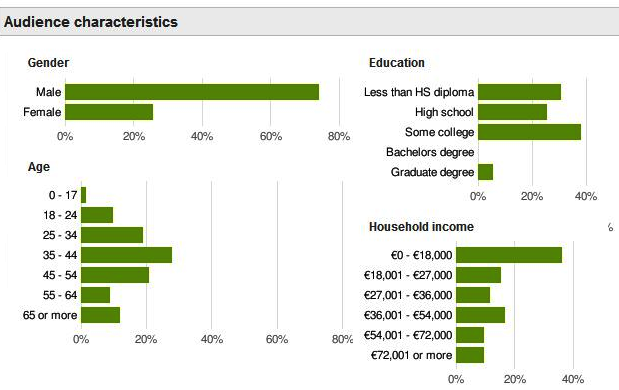
\includegraphics[scale=0.65]{../screenshots/ad-planner.png}
\caption{Ad-Planner Besucherstatistik (Beispiel)}
\label{abb:adplanner1}
\end{center}
\end{figure}

Die Grafik Bild \ref{abb:adplanner1} zur Besucherstatistik wurde vom Google Ad-Planner f�r eine (hier nicht genannte) Website erstellt. Man erkennt, das der �berwiegende Anteil der Besucher m�nnlich und zwischen 35-44 Jahre alt ist. (Die Informationen zu Bildung und Haushaltseinkommen m�ssen im Vergleich zu allgm. Statistiken der Bev�lkerung bewertet werden, was hier mal entf�llt.)\\

\textbf{Wie kommt das Imperium zu diesen Daten?} Es gibt so gut wie keine M�glichheit, diese Daten irgendwo einzugeben. Google fragt NICHT nach diesen Daten, sie werden aus der Analyse des Surf- und Suchverhaltens gewonnen. Zus�tzlich kauft Google bei Marktforschungsunternehmen gro�e Mengen an Informationen, die in die Kalkulation einflie�en.\\

Wenn jemand mit dem iPhone auf der Website von BMW die Preise von Neuwagen studiert, kann Google ihn einer Einkommensgruppe zuordnen. Wird der Surfer sp�ter beim Besuch von Spiegel-Online durch Einblendung von Werbung wiedererkannt, kommt ein entsprechender Vermerk in die Datenbank. Au�erdem kann die Werbung passend zu seinen Interessen und Finanzen pr�sentiert werden. (Die Realit�t ist nat�rlich etwas komplexer.)\\

Mit dem im April 2010 eingef�hrtem \textbf{Retargeting} geht Google noch weiter. Mit Hilfe spezieller Cookies werden detailierte Informationen �ber Surfer gesammelt. Die Informationen sollen sehr genau sein, bis hin zu Bekleidungsgr��en, f�r die man sich in einem Webshop interessiert hat. Die gesammelten Informationen sollen die Basis f�r punktgenaue Werbung bieten. Beispielsweise soll nach dem Besuch eines Webshops f�r Bekleidung ohne Kaufabschluss permanent alternative Werbung zu diesem Thema eingeblendet werden. 

\subsubsection*{Google Mail, Talk, News... und Google+ (personalisierte Dienste)}
Mit einem einheitlichem Google-Konto k�nnen verschiedene personalisierte Angebote genutzt werden. (Google Mail, News, Talk, Calendar, Alert, Orkut, B�rsennachrichten..... iGoogle)\\

Bei der Anmeldung ist das Imperium weniger wissbegierig, als vergleichbare kommerzielle Anbieter. Vor- und Nachname, Login-Name und Passwort reichen aus. Es ist nicht unbedingt n�tig, seinen realen Namen anzugeben. Ein Pseudonym wird auch akzeptiert. Die Accounts erm�glichen es, aus dem Surf- und Suchverhalten, den zusammengestellten Nachrichtenquellen, dem Inhalt der E-Mails usw. ein Profil zu erstellen. Die unsicher Zuordnung �ber allgemeine Cookies, IP-Adressen und andere Merkmale ist nicht n�tig.\\

Au�erdem dienen die Dienste als Fl�chen f�r personalisierte und gut bezahlte Werbung.\\

Patente aus dem Umfeld von Google Mail zeigen, dass dabei nicht nur Profile �ber die Inhaber der Accounts erstellt werden, sondern auch die Kommunikationspartner unter die Lupe genommen werden. Wer an einen Google Mail Account eine eMail sendet, landet in der Falle des Datenkraken.\\

Die Einrichtung eines Google-Accounts erm�glicht es aber auch, gezielt die gesammelten Daten in gewissem Umfang zu beeinflussen. Man kann Eintr�ge aus der Such- und Surf-Historie l�schen u.�. (Besser ist es sicher, die Eintr�ge von vornherein zu vermeiden.)

\subsubsection*{Kooperation mit Beh�rden und Geheimdiensten}
Es w�re verwunderlich, wenn die gesammelten Datenbest�nde nicht das Interesse der Beh�rden und Geheimdienste wecken w�rden. Google kooperiert auf zwei Ebenen:
\begin{enumerate}
 \item 
       
Auf Anfrage stellt Google den Beh�rden der L�nder die angeforderten Daten zur Verf�gung. Dabei agiert Google auf Grundlage der nationalen Gesetze. Bei daten-speicherung.de findet man Zahlen zur Kooperationswilligkeit des Imperiums. Durchschnittlich beantwortet Google Anfragen mit folgender H�ufigkeit:
\begin{itemize}
\item 3mal t�glich von deutschen Stellen
\item 20mal t�glich von US-amerikanischen Stellen
\item 6mal t�glich von britischen Stellen
\end{itemize}
\item Au�erdem kooperiert Google mit der CIA bei der Auswertung der Datenbest�nde im Rahmen des Projektes \textit{Future of Web Monitoring}, um Trends und Gruppen zu erkennen und f�r die Geheimdienste der USA zu erschlie�en. Es besteht der Verdacht, dass Google auch mit der NSA kooperiert. Das EPIC bem�ht sich, Licht in diese Kooperation zu bringen. Anfragen wurden bisher nicht beantwortet.
\end{enumerate}

\subsubsection*{Die (virtuelle) Welt ist eine ``Google'' - oder?}
Die vernetzten Rechenzentren von Google bilden den mit Abstand gr��ten Supercomputer der Welt. Dieser Superrechner taucht in keiner TOP500-Liste auf, es gibt kaum Daten, da das Imperium sich bem�ht, diese Informationen geheim zu halten. Die Datenzentren werden von (selbst�ndigen?) Gesellschaften wie Exaflop LLC betrieben.\\

Neugierige Journalisten, Blogger und Technologieanalysten tragen laufend neues Material �ber diese Maschine zusammen. In den Materialsammlungen findet man 12 bedeutende Anlagen in den USA und 5 in Europa, die als wesentliche Knotenpunkte des Datenuniversums eingesch�tzt werden. Weitere kleinere Rechenzentren stehen in Dublin, Paris, Mailand, Berlin, M�nchen Frankfurt und Z�rich. In Council Bluffs (USA), Thailand, Malaisia und Litauen werden neue Rechenzentren gebaut, die dem Imperium zuzurechnen sind. Das gr��te aktuelle Bauprojekt vermuten Journalisten in Indien. (2008)\\

Experten sch�tzen, dass ca. 1 Mio. PCs in den Rechenzentren f�r Google laufen (Stand 2007). Alle drei Monate kommen etwa 100 000 weitere PCs hinzu. Es werden billige Standard-Komponenten verwendet, die zu Clustern zusammengefasst und global mit dem \textit{Google File System (GFS)} vernetzt werden. Das GFS gew�hrleistet dreifache Redundanz bei der Datenspeicherung.\\

Die Kosten f�r diese Infrastruktur belaufen sich auf mehr als zwei Milliarden Dollar j�hrlich. (2007)\\

Die Videos von Youtube sollen f�r 10\% des gesamten Traffics im Internet verantwortlich sein. �ber den Anteil aller Dienste des Imperiums am Internet-Traffic kann man nur spekulieren.
\begin{center}
\textbf{Google dominiert unser (virtuelles) Leben.}                                          \end{center}
Dabei geht es nicht um ein paar Cookies sondern um eine riesige Maschinerie.

\subsection{User-Tracking}
Viele Dienste im Web nutzen die M�glichkeiten, das Surfverhalten zu verfolgen, zu analysieren und die gesammelten Daten zu versilbern. Die dabei entstehenden Nutzerprofile sind inzwischen sehr aussagekr�ftig. Wie das Wall Street Journal in einer Analyse beschreibt, k�nnen das Einkommen, Alter, politische Orientierung und weitere pers�nliche Daten der Surfer eingesch�tzt werden oder die Wahrscheinlichkeit einer Kreditr�ckzahlung. Haupts�chlich werden diese Daten f�r Werbung genutzt. Ein Onlin-Versand von Brautkleidern m�chte Frauen im Alter von 24-30 Jahren ansprechen, die verlobt sind. Das ist heute m�glich.\\

Eine weitere Analyse des Wall Street Journal nimmt die Firma Rapleaf n�her unter die Lupe. Diese Firma ist auf die Auswertung von Cookies spezialisiert. Neben den genannten Pers�nlichkeitsprofilen kann Rapleaf auch den realen Namen und viele genutzte E-Mail Adressen aufdecken. Diese Informationen werden meist durch Nutzung von Facebook o.� verraten.\\

H�ufig werden \textit{Werbeeinblendungen} f�r das User-Tracking genutzt. Die in Webseiten darstellte Werbung wird nur von wenigen Anbietern zur Verf�gung gestellt. Diese verwenden verschiedene M�glichkeiten, um Surfer zu erkennen, das Surfverhalten Website �bergreifend zu erfassen und anhand dieser Daten Nutzerprofile zu generieren. F�r die Auswertung werden nicht nur die besuchten Websites genutzt. Besonders aussagekr�ftig sind die Klicks auf Werbung. S. Guha von Microsoft und B. Cheng sowie P. Francis vom Max Planck Institute f�r Software Systeme beschreiben in einer wiss. Ver�ffentlichung, wie man homosexuelle M�nner anhand der Klicks auf Werbung erkennen kann. Das Verfahren kann f�r verschiedene Fragestellungen angepasst werden.\\

Neben Werbung und Cookies werden auch \textit{HTML-Wanzen} (so genannten \textit{Webbugs}) f�r das Tracking eingesetzt. Dabei handelt es sich um 1x1-Pixel gro�e transparente Bildchen, welche in den HTML-Code einer Webseite oder einer E-Mail eingebettet werden. Sie sind f�r den Nutzer unsichtbar, werden beim Betrachten einer Webseite oder �ffnen der E-Mail vom externen Server geladen und hinterlassenen in den Logs des Servers Spuren f�r eine Verfolgung des Surfverhaltens.\\

Au�erdem gibt es spezielle Tracking-Dienste wie Google Analytics, die oft mit Javascipt arbeiten.\\

Gesetzliche Schranken scheint man gro�fl�chig zu ignorieren. Die Universit�t Karlsruhe hat eine Studie ver�ffentlicht, die zu dem Ergebnis kommt, dass nur 5 von 100 Unternehmen im Internet geltende Gesetze zum Datenschutz respektieren. Der Nutzer ist also auf Selbstschutz angewiesen. 


\subsection{Geotagging}
Geotagging ist \textit{the next big thing} unter den Angriffen auf die Privatsph�re. Es geht um die Frage, wo wir etwas tun oder getan haben und welche Bewegungsmuster erkennbar sind. 
\begin{enumerate}
 \item \textbf{Standortdaten} sind die wertvollsten Informationen f�r die Werbe�wirtschaft, um zuk�nftig den Markt zu vergr��ern. Ein Online-Versand von Brautkleidern richtet seine Werbung an Frauen zwischen 24-30 Jahren, die verlobt sind. Ein Ladengesch�ft stellt zus�tzlich die Bedingung, das sie sich h�ufig im Umkreis von xx aufhalten. Gezielte lokalisierte Werbung ist ein Markt, der durch die Verbreitung von Smartphones stark w�chst.
\item Die \textbf{Bewegungsanalyse} erm�glicht Aussagen �ber sehr private Details. Man kann z.B. durch die Analyse der Handybewegungen erkennen, ob jemand als Gesch�ftsreisender h�ufig unterwegs ist, ob man ein festes Arbeitsverh�ltnis hat, f�r welche Firma man t�tig ist oder ob man arbeitslos ist. Die Firma Sense Networks ist ein Vorreiter auf dem Gebiet der Bewegungsanalyse. Im Interview mit \textit{Technology Review} beschreibt Greg Skibiski seine Vision:
\begin{quote}
\textit{Es entsteht ein fast vollst�ndiges Modell. Mit der Beobachtung dieser Signale kann man ganze Firmen, ganze St�dte, eine ganze Gesellschaft r�ntgen. }
\end{quote}
\href{http://www.heise.de/tr/artikel/Immer-im-Visier-276659.html}{http://www.heise.de/tr/artikel/Immer-im-Visier-276659.html}\\

Das Magazin Wired berichtete im Danger Room (Oktober 2011), dass das FBI Smartphones bereits seit Jahren mit dieser Zielstellung der "Durchleuchtung der Gesellschaft" trackt. Muslimisch Communities werden systematisch ananlysiert, ohne dass die betroffenen Personen im Verdacht einer Straftat stehen. Das Geotracking von GPS-f�higen Smartphones und GPS-Modulen moderner Fahrzeuge durch das FBI erfolgt ohne richterlichen Beschluss.
\begin{quote}
  \textit{\dots the pushpins on the new FBI geo-maps indicate where people live, work, pray, eat and shop, not necessarily where they commit or plan crimes.}
\end{quote} 
\href{http://www.wired.com/dangerroom/2011/10/fbi-geomaps-muslims/}{http://www.wired.com/dangerroom/2011/10/fbi-geomaps-muslims}
\end{enumerate}
\subsubsection*{Datensammlung}
 Die Daten werden mit verschiedenen Methoden gesammelt: 
\begin{itemize}
\item Hauptlieferanten f�r Geodaten sind Smartphones und Handys. Vor allem Apps k�nnen genutzt werden, um Geodaten zu sammeln. V�ber die H�lfte der in verschiedenen Stores downloadbaren Apps versenden Stand�ortdaten unabh�ngig davon, ob sie f�r die Funktion der App n�tig sind. Der Bundes�daten�schutz�beauftragte erw�hnt beispiels�weise eine App, die das Smartphone zur Taschenlampe macht und dabei den Standort an den Entwickler der App sendet.\\

\item Mit Einf�hrung des iPhone 4 hat Apple seine Datenschutzbestimmungen ge�ndert. Die gesamte Produktpalette von Apple (iPhone, Laptops, PC\dots) wird in Zukunft den Standort des Nutzers laufend an Apple senden. Apple wird diese Daten Dritten zur Verf�gung stellen. Wer Zugang zu diesen Daten hat, wird nicht n�her spezifiziert. \href{http://www.apple.com/chde/legal/privacy/}{http://www.apple.com/chde/legal/privacy/}\\

F�r die Datensammlungen rund um das iPhone wurde Apple mit dem BigBrother Award 2011 geehrt. Auszug aus der Laudation von F. Rosengart und A. Bogk:
\begin{quote}
\textit{Apples Firmenstrategie scheint darauf ausgelegt zu sein, m�glichst viele Daten der Nutzer zu erfassen, �hnlich wie es soziale Netzwerke auch tun. Werbepartner freuen sich darauf, mit Hilfe von Apple m�glichst zielgruppengerechte und standortbezogene Werbung auf dem Telefon anzeigen zu k�nnen.}
\end{quote} 

\item Millionen von Fotos werden �ber verschiedene Dienste im Internet ver�ffentlicht (Flickr, Twitter, Facebook\dots). H�ufig enthalten diese Fotos in den EXIF-Attributen die GPS-Koordinaten der Aufnahme. Die Auswertung dieses Datenstromes steht erst am Anfang der Entwicklung. Ein Beispiel ist die Firma Heypic, die mit Risikokapital ausgestattet die Fotos von Twitter durchsucht und auf einer Karte darstellt.

\item Die ganz normale HTTP-Kommunikation liefert Standortinformationen anhand der IP-Adresse. Aktuelle Browser bieten zus�tzlich eine Geolocation-API, die genauere Informationen zur Verf�gung stellt. Als Facebook im Sommer 2010 die Funktion Places standardm��ig aktivierte, waren viele Nutzer �berrascht, wie genau jede reale Bewegung im Sozialen Netz lokalisiert wird. (Nicht nur Facebook kann das.)\\

\begin{figure}[htb]
\begin{center}
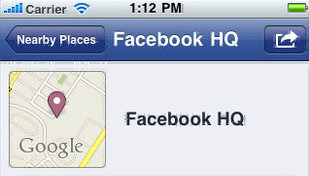
\includegraphics[scale=0.55]{../screenshots/facebook1.png}
\caption{Lokalisierung eines Smartphone durch Facebook}
\label{abb:facebook1}
\end{center}
\end{figure}

Die Deaktivierung von Places scheint bei Facebook wirklich umst�ndlich zu sein. Damit wird aber nicht die Erfassung der Daten deaktiviert, sondern nur die Sichtbarkeit f�r andere Nutzer!

\item Lokalisierungsdienste wie \textit{Gowalla} oder \textit{Foursquare} bieten �ffentlich einsehbare Standortdaten und versuchen, durch spielartigen Charakter neue Nutzer zu gewinnen. Im Gegensatz zu den oben genannten Datensammlungen kann man bei Gowalla oder Foursquare aber gut kontrollieren, welche Daten man ver�ffentlicht oder die Dienste nicht nutzen.
\end{itemize}

\newpage
\section{Ein Konzept f�r spurenarmes Surfen}

Das auf den folgenden Seiten vorgestellte Konzept zum spurenarmen Surfen umfasst folgende Punkte:

\begin{enumerate}
\item Die Nutzung datensammelnder Webangebote kann man vermeiden.
\item Die Annahme von Cookies und die Ausf�hrung von JavaScript wird auf vertrauensw�rdige Websites eingeschr�nkt.
\item Werbung, HTML-Wanzen und die Like-Buttons (mit denen Social Networks wie Facebook Daten sammeln) werden durch Filter blockiert.
\item Verr�terische Informationen des Browsers werden entfernt.
\item Risikoreiche und Privacy-unfreundliche Features wie PDF-Reader Plug-Ins, Browser History, Geolocation usw. werden im Browser deaktiviert.
\item HTTPS-Zertifikate werden zus�tzlich validiert, um Man-in-middle Angriffe zu erschweren.
\item Der Datenverkehr kann �ber einen Anonymisierungsdienst geleitet werden. Die verschl�sselte Kommunikation verhindert auch die Auswertung des Internetverkehrs durch mitlesende Dritte wie z.B. unsichere WLAN-Hotspots oder TK�V. (siehe \textit{Anonymymisierungsdienste nutzen})
\end{enumerate}

Mit diesen Ma�nahmen kann es vorkommen, dass Websites nicht wie erwartet funktionieren. Gute Webdesigner verzichteten auf suspekte Technologien, JavaScript wird sinnvoll eingesetzt und der Surfer auf fehlende Freigaben hingewiesen. Cookies sind meist f�r Logins n�tig und Javascript erm�glicht h�bsche Animationen oder Pr�fung von Eingaben.

\begin{center}

\includegraphics[scale=0.75]{../screenshots/cookies_required1.png}
\end{center}

Weniger gute Webseiten liefern seltsame Fehlermeldungen:

\begin{center}
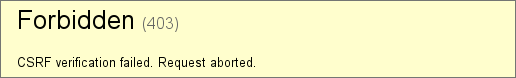
\includegraphics[scale=0.75]{../screenshots/cookies_wrong1.png}
\end{center}

Ganz schlechte Websites machen irgendwas, aber nicht was man erwartet Gelegentlich werden auch Referer oder User-Agent ausgewertet, obwohl es belanglos sein sollte, und Surfer werden nicht auf die notwendigen Freigaben hingeweisen. Hier ist man auf Probieren und Raten angewiesen. Als erstes kann man Cookies freigeben. Wenn das hilft kann man Javascript gezielt f�r einzelne Server freigeben. Ob die Deaktivierung der Schutzma�nahmen die volle Funktionalit�t aufwiegt, muss man bei Bedarf selbst entscheiden.\\

\section{Auswahl des Webbrowsers}
Firefox ist der Webbrowser der Mozilla Foundation. Er ist kostenfrei nutzbar und steht auf der Website des Projektes \footnote{ \href{http://www.mozilla-europe.org/de/firefox}{http://www.mozilla-europe.org/de/firefox}} f�r fast alle Betriebssystem zum Download bereit. Linux-Distributionen enthalten den Browser in der Regel.\\

Debian GNU/Linux enth�lt eine branded version des Browsers unter dem Namen \textit{Iceweasel}, allerding oft in einer veralteten Version. Das Mozilla Debian Team stellt eine aktuelle Version in einem extra Repository \footnote{ \href{http://mozilla.debian.net}{http://mozilla.debian.net}} bereit.\\

Firefox kann durch viele von der Community entwickelte Add-ons und Anpassungen in der Konfiguration zu einem sicheren und privacy-freundlichen Browser aufgewertet werden. Ich beschr�nke mich im folgenden auf diesen einen Browser. Das ist schon sehr umfangreich, wenn man es gut machen will.

\subsubsection*{JonDoFox}
Der JonDoFox\footnote{ \href{https://www.anonym-surfen.de/jondofox.html}{https://www.anonym-surfen.de/jondofox.html}} ist ein Browser-Profil f�r Firefox, dass alle Einstellungen umsetzt, die auf den folgenden Seiten beschrieben werden. Nach der Installation von Mozilla Firefox ist das JonDoFox-Profil zus�tzlich zu installieren - fertig. Zuk�nftig fragt Firefox bei jedem Start, welches Profil genutzt werden soll. JonDoFox ist f�r anonymes Surfen mit JonDonym entwickelt worden, kann aber auch ohne Anonymisierungsdienst verwendet werden, indem man in der Statuszeile unten rechts auf \textit{Kein Proxy} oder \textit{Benutzerdefiniert} umschaltet.

\begin{center}
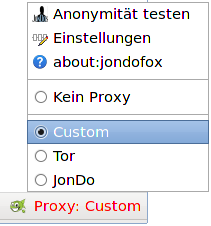
\includegraphics[scale=0.75]{../screenshots/jondofox-proxy-ohne.png}
\end{center}

Wenn man den Proxy \textit{Benutzerdefiniert} w�hlt, kann die User-Agent Kennung modifiziert werden. Das ist vor allem f�r Nutzer seltener Betriebssysteme sinnvoll, um sich in der Masse der Windows-Nutzer zu verstecken. In den Einstellungen des JonDoFox kann man f�r Benutzerdefinierte Proxys den \textit{Firefox 17.0 f�r Windows} (JonDo) oder \textit{Firefox 10.0 f�r Windows} (Tor) als Fake zu nutzen. Mit dieser kleinen Anpassung erh�lt man einen optimal konfigurierten Browser. Das folgende Kapitel kann man trotzdem lesen oder �berfliegen, um die damit verbundenen Einschr�nkungen besser zu verstehen.\\

\begin{figure}[htb]
\begin{center}
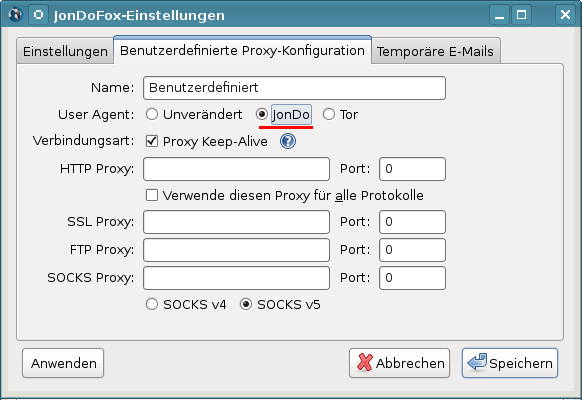
\includegraphics[scale=0.7]{../screenshots/jondofox-ua-ohne.png}
\caption{User-Agent Kennung konfigurieren}
\label{abb:jondofox-ua}
\end{center}
\end{figure}

Eine kurze Einf�hrung in den Umgang mit JonDoFox gibt es im Kapitel Anonymisierungsdienste.

\subsubsection*{JoDoBrowser}
Der JonDoBrowser\footnote{ \href{https://www.anonym-surfen.de/jondobrowser.html}{https://www.anonym-surfen.de/jondobrowser.html}} ist nicht nur sicher konfiguriert sondern enth�lt auch Modifikationen im Source Code von Mozilla Firefox, um eine h�here Anonymit�t zu bieten. Die aktuelle Beta Version arbeitet stabil und kann meiner Meinung nach f�r die t�gliche Arbeit eingesetzt werden.\\

Standardm��ig ist die Proxy-Umschaltung im JonDoBrowser deaktiviert. Das erweiterte Men� muss erst in den Einstellungen des JonDoFox-XPI (siehe Bild \ref{abb:proxyfreigeben}) aktiviert werden. Dann kann man wie beim JonDoFox auf \textit{``Kein Proxy``} umschalten und ohne Anonymisierungsdienst spurenarm surfen.

\begin{figure}[htb]
\begin{center}
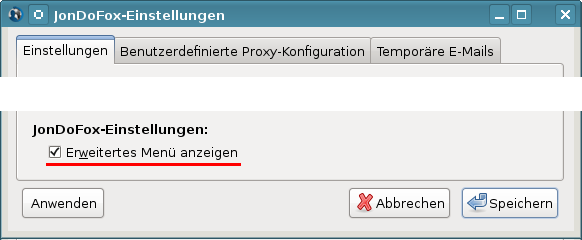
\includegraphics[scale=0.7]{../screenshots/jondobrowser-proxy-aktivieren.png}
\caption{Proxy-Umschaltung im JonDoBrowser freigeben}
\label{abb:proxyfreigeben}
\end{center}
\end{figure}
\section{Datensparsame Suchmaschinen}
Suchmaschinen werden sicher am h�ufigsten genutzt, um sich im Web zu orientieren. Neben den bekannten Datensammlern wie Google, MSN oder Yahoo gibt es durchaus Alternativen.\\

\subsubsection*{Suchmaschinen mit eigenem Index}
Es ist nicht einfach, eine Suchmaschine zu finden, die die Privatsph�re der Nutzer respektiert, einen umfangreichen Index zur Verf�gung stellt und gute Ergebnisse liefert. Ein paar Vorschl�ge:
\begin{itemize}
\item \textbf{DuckDuckGo.com} (\href{https://duckduckgo.com}{https://duckduckgo.com})\\
ist eine privacyfreundliche Suchmaschine. Es gibt sie in einer Java�script-freien Version (HTML) und mit Javascript. Wenn Javascript freigegeben ist, werden an der rechten Seite unter \textit{Search suggestions} Vorschl�ge f�r die Eingrenzung der Suche auf bestimmte Cluster angezeigt.\\

\begin{figure}[tb]
\begin{center}
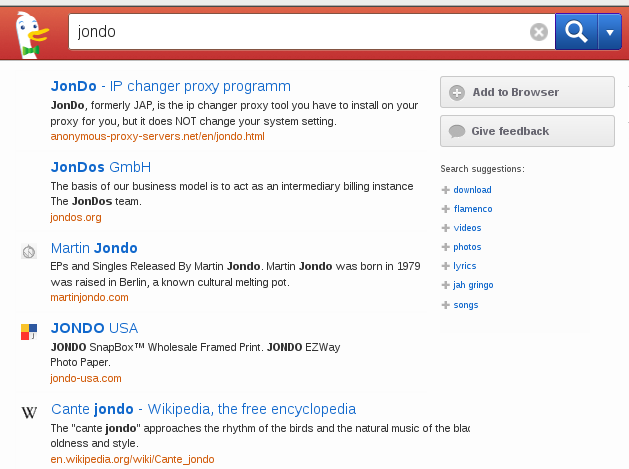
\includegraphics[scale=0.75]{../screenshots/duckduckgo.png}
\caption{Suchergebnisse bei DuckDuckGo mit Search suggestions}
\label{abb:ddgsuche}
\end{center}
\end{figure}

Bei der Suche nach ``jondo`` im Bild \ref{abb:ddgsuche} kann man bspw. die Ergebnisse auf Downloads begrenzen (wenn man nach dem Anonymierungs-Proxy sucht), auf Songs oder Lyrik (wenn man sich �ber den S�nger Martin JonDo informieren will) oder auf Flamenco (wenn man mehr Ergebnisse zum Cante jondo haben m�chte). Dieses Feature ist eine gute Kompensation f�r die nicht vorhandene Personalisierung.\\

Die Javascripte enthalten keinen Tracking Code. F�r diese Webseite kann ich die dauerhafte Freigabe von Javascript empfehlen.\\

Neben der eigentlichen Suche bietet DuckDuckGo viele nette Erweiterungen \footnote{ \href{https://duckduckgo.com/goodies.html}{https://duckduckgo.com/goodies.html}}. Das Suchfeld kann als Taschenrechner genutzt werden, Einheiten k�nnen umgerechnet werden, Fragen nach dem Wetter k�nnen beantwortet werden (in englisch: \textit{weather} oder \textit{is it raining})\dots u.v.a.m.

\item \textbf{Blekko} (\href{https://blekko.com/}{https://blekko.com})\\
Blekko hatte als erste Suchmaschine eine gute L�sung gegen Spam. Allerdings bietet sie keine Einschr�nkung auf bestimmte Sprachen. In den Ergebnissen dominieren englische Seiten. Die IP-Adressen der Nutzer werden nach 48h gel�scht.

\item \textbf{Open Directory} (\href{http://www.dmoz.de/}{http://www.dmoz.de} oder \href{http://www.dmoz.org/}{http://www.dmoz.org})\\
Das Open Directory ist ein Katalog, der von Freiwilligen gepflegt wird. Man kann die Suche auf Kategrien eingrenzen und erh�lt �bersichtliche Ergebnislisten.
\end{itemize}
Beide Suchmaschinen bieten gute Ergebnisse bei einfachen Suchanfragen. Komplexe Suchanfragen mit mehreren Begriffen beantwortet Google oder die als Google-Proxy nutzbaren Suchmaschine \textbf{Startpage} besser.

\subsubsection*{Meta-Suchmaschinen}
Meta-Suchmaschinen leiten die Suchanfrage an mehrere Suchdienste weiter. Sie sammeln die Ergebnisse ein und sortieren sie neu.
\begin{itemize}
 \item \textbf{Ixquick.com} (\href{https://www.ixquick.com/deu/}{https://www.ixquick.com/deu})\\
wird von der niederl�ndischen Firma Surfboard Holding B.V. betrieben. Die Suchmaschine speichert keine IP-Adressen und generiert keine Profile der Nutzer. Diese Meta-Suche fragt mehrere externe Suchmaschinen an, aber nicht Google. Ixquick.com ist mit dem Datenschutzsiegel EuroPriSe zertifiziert.\\

Als kleines Schmankerl bietet Ixquick die M�glichkeit, aus den Suchergebnissen heraus die Webseiten �ber einen anonymisierenden Proxy aufzurufen. Die aufgerufene Webseite sieht damit nur eine IP-Adresse von Ixquick. Neben den Ergebnissen findet man einen kleinen Link \textit{Proxy}: 
\begin{center}
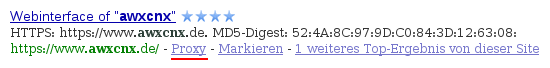
\includegraphics[scale=0.75]{../screenshots/ixquick.png}
\end{center}

Aus Sicherheitsgr�nden entfernt der Proxy Javascript Code aus den aufgerufenen Webseiten. Es ist daher m�glich, dass einige Webseiten nicht wie erwartet funktionieren. Au�erdem ist KEINE Eingabe von Daten in Textfeldern der aufgerufenen Webseite m�glich. Der Proxy kann die Webseiten nur darstellen.

\item \textbf{Startpage} (\href{https://startpage.com/}{https://startpage.com})\\
wird ebenfalls von Surfboard Holding B.V. betrieben und ist mit dem Datenschutzsiegel EuroPriSe zertifiziert. Die Suchmaschine bietet privacy-freundlichen Zugriff auf die Google-Suche, ist also einen ideale Erg�nzung zu Ixquick.com. Einen Proxy zum anonymen Aufruf der Webseiten aus den Ergebnissen bietet Startpage auch.

\item \textbf{Metager2.de} (\href{http://www.metager2.de/}{http://www.metager2.de})\\
ist ein Klassiker vom Suma e.V. Neben klassischen Suchdiensten wird auch die Peer-2-Peer Suche Yacy einbezogen. Dadurch verz�gert sich die Anzeige der Ergebnisse etwas.
\end{itemize}

\subsubsection*{Spezielle Anwendungsf�lle}
\begin{itemize}
 \item Wikipedia kann man auch ohne Umweg �ber Google direkt fragen, wenn man Informationen sucht, die in einer Enzyklop�die zu finden sind.
 \item Statt Google �bersetzen zu lassen, kann man LEO nutzen. Der Translator kennt neben Englisch und Deutsch weitere Sprachen.
\end{itemize}

\subsubsection*{Peer-2-Peer Suchmaschine}
Yacy \footnote{ \href{http://yacy.net/}{http://yacy.net}} ist eine zensurresistente Peer-2-Peer Suchmaschine. Jeder kann sich am Aufbau des Index beteiligen und die Software auf seinem Rechner installieren. Der Crawler ist in Java geschrieben, ben�tigt also eine Java-Runtime (JRE), die es f�r WINDOWS bei Oracle \footnote{ \href{http://java.sun.com}{http://java.sun.com}} zum kostenlosen Download gibt. Linuxer k�nnen das Paket \textit{default-jre} mit der Softwareverwaltung installieren. Danach holt man sich die Yacy-Software von der Website des Projektes und startet den Installer - fertig. F�r Debian, Ubuntu und Linux Mint bietet das Projekt ein Repository  \footnote{ \href{http://www.yacy-websuche.de/wiki/index.php/De:DebianInstall}{http://www.yacy-websuche.de/wiki/index.php/De:DebianInstall}} mit fertigen Paketen.\\

Nach dem Start von Yacy kann man im sich �ffnenden Bowserfenster die Basiskonfiguration anpassen und los gehts. Die Suchseite ist im Browser unter \href{http://localhost:8080}{http://localhost:8080} erreichbar.\\

Die Beantwortung der Suchanfragen dauert mit 5-10sec ungewohnt lange. Au�erdem muss Javascript f�r \textit{http://localhost} freigegeben werden, damit die Ergebisseite sauber dargestellt wird. Mit den Topwords unter den Ergebnissen bietet Yacy ein Konzept, um die Suchanfrage zu pr�zisieren.\\

F�r alle alternativen Suchmaschinen gilt, dass sie eine andere Sicht auf das Web bieten und die Ergebnisse sich von Google unterscheiden. Man sollte bei der Beurteilung der Ergebnisse beachten, dass auch Google nicht die reine Wahrheit bieten kann, sondern nur eine bestimmte Sicht auf das Web.

\subsubsection*{Google ???}
Anfang Februar 2012 hat Google seine Suchmaschine �berarbeitet. Die Webseite macht jetzt intensiven Gebrauch von Javascript. Eine vollst�ndige Analyse der verwendeten Sch�ffel�techniken liegt noch nicht vor. Einige vorl�ufige Ergebnisse sollen kurz vorgestellt werden:

\begin{description}
 \item[Einsatz von EverCookies:] Der Surfer wird mit EverCookie Techniken markiert. Die Markierung wird im DOMStorage gespeichert. Der DOMStorage wurde vom W3C spezifiziert, um Web-Applikationen die lokale Speicherung gr��erer Datenmengen zu erm�glichen und damit neue Features zu erschlie�en. Google wertet die User-Agent Kennung und weitere Informationen �ber den Browser aus, um die M�glichkeit der Nutzung des DOMStorage erst einmal zu pr�fen und gegebenenfalls Alternativen wie normale Cookies zu verwenden.

\item[Tracking der Klicks auf Suchergebnisse:] Bei Klick auf einen Link in den Suchergebnissen wird die Ziel-URL umgeschrieben. Aus der f�r den Surfer sichtbaren Zieladresse 
\begin{verbatim}
  https://www.awxcnx.de/handbuch.htm 
\end{verbatim} 

wird im Moment des Klick eine Google-URL: 
\begin{verbatim}
  http://www.google.de/url?q=https://www.awxcnx.de/...... 
\end{verbatim} 

Die zwischengeschaltete Seite enth�lt eine 302-Weiterleitung auf die urspr�ngliche Ziel-URL. Der Surfer wird also fast unbemerkt �ber einen Google-Server geleitet, wo der Klick registriert wird. (Bei deaktiviertem Javascript ist stets die Google-URL sichtbar, nicht die Zieladresse.)\\

Diese Umschreibung der Links gibt es auch bei Bing, Facebook, Youtube und anderen Daten�sammlern. Das Firefox Add-on Google Privacy kann diese Umschreibung verhindern. Das Add-on ist noch im Beta Status. Die Entwicklung von \textit{Google Privacy} ist ein Wettlauf zwischen Hase und Igel. Einfacher und sicherer ist es, privacy freundliche Suchmaschinen zu nutzen.

\item[Browser Fingerprinting:] Mittels Javascript wird die innere Gr��e des Browserfensters ermittelt. Folgenden Code findet man in den Scripten:
\begin{verbatim}
 I[cb].oc= function() {
 var a=0, b=0;
 self.innerHeight?(a=self.innerWidth,b=self.innerHeight):....;
 return {width:a, height:b}
 };
\end{verbatim} 

Die ermittelten Werten werden als Parameter \textit{biw} und \textit{bih} in der Google-URL �bergeben. Sie haben aber keinen Einfluss auch die Bildschirmdarstellung. Auch wenn das Browserfenster zu klein ist und die Darstellung nicht passt, bleiben die festen Gr��en der HTML-Elemente erhalten.\\

Die inneren Abmessungen des Browserfensters sind sehr individuelle Parameter, der von Betriebssystem und gew�hlten Desktop-Einstellungen abh�ngig sind. Sie werden von der Schriftgr��e in der Men�leiste, der Fensterdekoration, den aktivierten Toolbars der Desktops bzw. der Browser usw. beeinflusst. Sie sind f�r die Berechnung eines individuellen Fingerprint des Browsers gut geeigent. Anhand des Browser-Fingerprint k�nnen Surfer auch ohne Cookies oder EverCookies wiedererkannt werden. Die Google Technik kann dabei besser differenzieren als das Projekt Panopticlick der EFF, das berets 80\% der Surfer eindeutig identifizieren konnte.
 \end{description}

Auf der Webseite der Google-Suche kann man dem Tracking kaum entgehen. Wer unbedingt die Ergebnisse von Google braucht, kann die Suchmaschine \textit{Startpage.com} als anonymisierenden Proxy nutzen. Sie ist mit dem Datenschutzsiegel EuroPriSe zertifiziert. Andere Suchmaschinen bieten eine andere Sicht auf das Netz - auch nicht schlecht, erfordert aber etwas Umgew�hnung.



\subsection{Firefox konfigurieren}
Am einfachsten installiert man ein Plug-In f�r die Suchleiste von Firefox, indem man die Web�seite der Suchmaschine aufruft und die Liste der Suchmaschinen ausklappt. Am Ende der Liste findet man das Plug-In f�r diese Suchmaschine, das man mit einem Klick hinzuf�gen kann.\\
\begin{figure}[tb]
\begin{center}
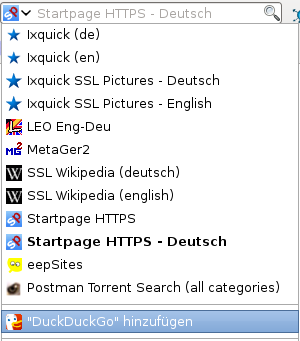
\includegraphics[scale=0.75]{../screenshots/suchmaschine-install.png}
\caption{Suchmaschine DuckDuckGo hinzuf�gen}
\label{abb:ffsucheadd}
\end{center}
\end{figure}

F�r viele Suchdienste gibt es Plug-Ins zur Integration in die Suchleiste von Mozilla Firefox bei mycroft.mozdev.org\footnote{ \href{http://mycroft.mozdev.org/}{http://mycroft.mozdev.org/}}. In einem Suchformular gibt man den Namens der Suchmaschine ein und findet schnell ein umfangreiche Liste von Varianten. Ein Klick in der Liste der Ergebnisse installiert das Plug-In in der Suchleiste. (Die Installation funktioniert nur mit JavaScript.)\\

F�r viele Suchmaschinen wie DuckDuckGo, Ixquick, Google, Wikipeadia, Startingpage u.a.m. gibt es eine Variante mit SSL-Verschl�sselung. Diese Variante sollte bevorzugt werden.\\

Au�erdem kann die Generierung von Suchvorschl�gen deaktiviert werden. Die Vorschl�ge kommen von dem gew�hlten Suchdienst, verlangsamen aber die Reaktion auf Eingaben deutlich. Ich weiss selber, was ich suche!  Den Dialog findet man unter \textit{Suchmaschinen verwalten} in  der Liste der Suchmaschinen.

\begin{figure}[tb]
\begin{center}
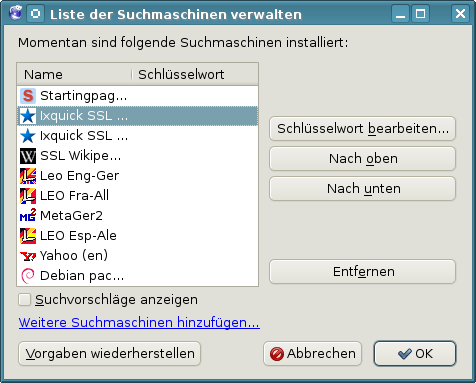
\includegraphics[scale=0.75]{../screenshots/firefox_suche.png}
\caption{Suchmaschinen verwalten}
\label{abb:ffsuche}
\end{center}
\end{figure}

\section{Cookies}
Cookies werden f�r die Identifizierung des Surfers genutzt. Neben der erw�nschten Identifizierung um personalisierte Inhalte zu nutzen, beispielsweise einen Web-Mail-Account oder um Eink�ufe abzuwickeln, werden sie auch f�r das Tracking von Nutzern verwendet.\\

Der Screenshot Bild \ref{abb:cookiespiegel} zeigt die Liste der Cookies, die bei einem einmaligen Aufruf der Seite \textit{www.spiegel.de} gesetzt wurden. Neben den Cookies von \textit{spiegel.de} zur Z�hlung der Leser setzen gleich mehrere datensammelnde Werbeserver Cookies und au�erdem Z�hldienste (quality-chanel.de, ivwbox.de), welche die Reichweiten von Online-Publikationen auswerten.\\

\begin{figure}[p]
\begin{center}
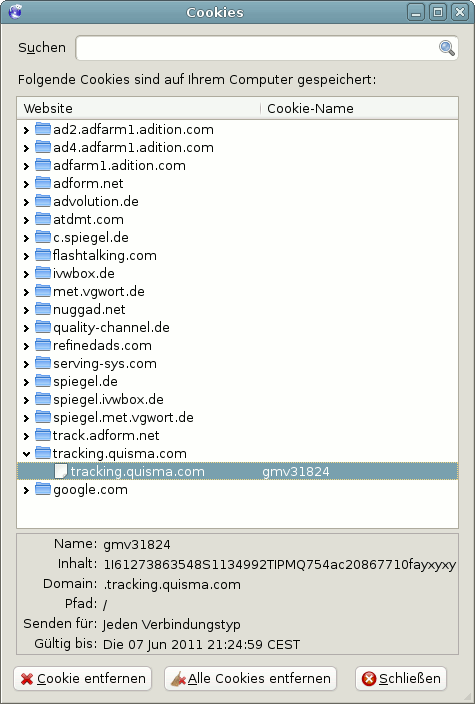
\includegraphics[scale=0.75]{../screenshots/cookies_spiegel.png}
\caption{Liste der Cookies beim Besuch von Spiegel-Online}
\label{abb:cookiespiegel}
\end{center}
\end{figure}

Es ist nicht ungew�hnlich, dass popul�re Webseiten mehrere Datensammler einbinden. Eine Studie der Universit�t Berkeley \footnote{ \href{http://heise.de/-1288914}{http://heise.de/-1288914}}  hat 2011 beim Surfen auf den TOP100 Webseiten 5.675 Cookies gefunden (ohne Login oder Bestellung). 4.914 Cookies wurden von Dritten gesetzt, also nicht von der aufgerufenen Webseite. Die Daten wurden an mehr als 600 Server �bermittelt. Spitzenreiter unter den Datensammlern ist Google, 97\% der popul�ren Webseiten setzen Google-Cookies.\\

Sinnvoll ist ein \textbf{Whitelisting} f�r die Behandlung von Cookies:

\begin{enumerate}
\item Standardm��ig wird die Annahme von Cookies verweigert.
\item F�r vertrauensw�rdige Websites, welche die Nutzung von Cookies zur Erreichung der vollen Funktion ben�tigen, werden Ausnahmen zugelassen.
\item Die f�r den Zugriff auf personalisierte Inhalte gespeicherten Cookies sollten beim Schlie�en des Browsers automatisch gel�scht werden. Einige Websites verwenden diese Cookies auch nach dem Logout f�r das User-Tracking.
\end{enumerate} 

Fast alle Login-Seiten, welche Cookies zur Identifizierung des Surfers verwenden, weisen mit einem kleinen Satz auf die notwendigen Freigaben hin. Treten beim Login seltsame Fehler auf, z.B. st�ndig die Fehlermeldung \textit{FALSCHES PASSWORT}, verweigert der Browser wahrscheinlich die Annahme von Cookies. Die Website sollte in die Liste der vertrauensw�rdigen Websites aufgenommen werden.\\



\subsection{Mozilla Firefox konfigurieren}
Mozilla Firefox bietet bereits standardm��ig die M�glichkeit, die meisten Cookies ohne Einbu�en am Surf-Erlebnis loszuwerden. Im Bild \ref{abb:cookiesff} gezeigte Dialog \textit{Einstellungen} Sektion \textit{Datenschutz} kann die Annahme von Fremd-Cookies standardm��ig deaktiviert werden.\\

\begin{figure}[htb]
\begin{center}
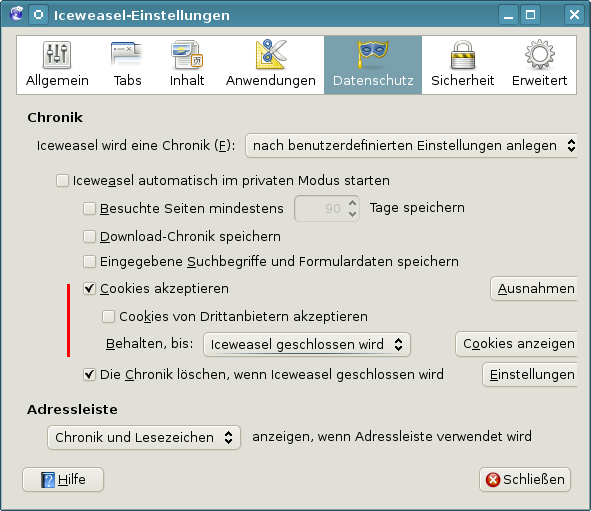
\includegraphics[scale=0.75]{../screenshots/CookiesFF.png}
\caption{Cookies-Einstellungen in Firefox}
\label{abb:cookiesff}
\end{center}
\end{figure}

Mit einem Klick auf den Button \textit{Ausnahmen} kann man Server konfigurieren, die Cookies setzen d�rfen oder grunds�tzlich blockiert werden. Um von Google nicht beim Besuch der meisten deutschen Websites verfolgt zu werden, ist es n�tig, diesen Dienst ausdr�cklich zu blockieren.\\

Anderenfalls wird der Browser beim Start durch den Aufruf der Default-Seite oder beim Laden der Phishing-Datenbank mit einem Google-Cookie ``personalisiert''. Durch eingebettete Werbung und Google-Analytics auf vielen Websites kann Google unbedarfte Surfer effektiv beobachten.

\subsubsection*{Zus�tzliche Add-ons f�r Firefox}
Die Firefox Addon Sammlung bietet viele Add-ons um die Verwaltung von Cookies zu erleichtern. Nicht alle werden noch gepflegt und sind mit aktuellen Versionen von Firefox kompatibel. Das Add-on \textbf{CookieMonster} \footnote{ \href{https://addons.mozilla.org/de/firefox/addon/cookie-monster/}{https://addons.mozilla.org/de/firefox/addon/cookie-monster/}} ist empfehlenswert. Es erlaubt die site-spezifische Verwaltung von Cookies.\\

Ein einfacher Klick auf das Install-Symbol der Website startet den Download der Erweiterung und installiert sie. Nach dem Neustart von Firefox ist in der Statusleiste ein zus�tzliches Symbol vorhanden. Ein Klick mit der linken(!) Maustaste auf das blau-schwarze ``CM`` �ffnet das in Bild \ref{abb:cookiesafe_1} dargestellte Men� (nur wenn die Website Cookies nutzen m�chte).

\begin{figure}[htb]
\begin{center}
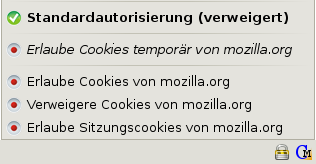
\includegraphics[scale=0.75]{../screenshots/Cookies1.png}
\caption{CookieMonster Men�}
\label{abb:cookiesafe_1}
\end{center}
\end{figure}

\begin{description}
\item[Erlaube Cookies tempor�r] erlaubt es dem aktuellen Server, nur f�r diese Sitzung Cookies zu setzen. Mit dem Schlie�en des Browsers werden die Cookies und die Ausnahme�reglung gel�scht.
\item[Erlaube Cookies] erlaubt es dem aktuellen Server, unbegrenzt g�ltige Cookies zu setzen. Diese Variante wird nur ben�tigt, wenn man bei einem sp�teren Besuch der Website automatisch wieder angemeldet werden m�chte.
\item[Verweigere Cookies] erlaubt es dem aktuellen Server nicht, Cookies zu setzen.
\item[Erlaube Sessioncookies] erlaubt es dem aktuellen Server, Cookies zu setzen. Mit dem Schlie�en des Browsers werden diese Cookies wieder gel�scht. Bei folgenden Besuchen d�rfen wieder neue Cookies gesetzt werden.
\end{description}

Nach der Installation von CookieMonster muss man das Standardverhalten auf \textit{Alle Cookies blockieren} umschalten. Das ist sicherer, als nur die Cookies von Dritt-Seiten zu blockieren. Die Einstellungen werden im Add-ons-Manager unter \textit{Extras -> Add-ons} in der Sektion \textit{Erweiterungen} konfiguriert.

\begin{figure}[htb]
\begin{center}
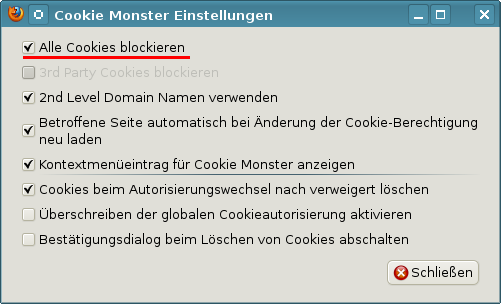
\includegraphics[scale=0.75]{../screenshots/CookiesFF2.png}
\caption{CookieMonster Einstellungen}
\label{abb:cookiesafe_2}
\end{center}
\end{figure}

\subsection{Super-Cookies in Firefox}
Mozilla Firefox bietet auch die clientseitige Datenspeicherung. Dieser DOM-Storage oder Web-Storage wird gelegentlich auch als Super-Cookie bezeichnet, da bis zu 5 MB gro�e Datenmengen mit Hilfe von Javascript abgelegt werden k�nnen.\\

Aktuelle Versionen von Firefox wenden die Beschr�nkungen f�r Cookies auch auf den DOMStorage an. Es reicht aus, die Cookies zu deaktivieren. Damit ist auch die clientseitige Datenspeicherung deaktiviert.\\

Diese parallele Anwendung der Einstellung f�r Cookies auf DOMStorage gilt nur f�r Firefox. Andere Browser verhalten sich bez�glich der clientseitigen Datenspeicherung anders! Bei Opera habe ich noch keine M�glichkeit gefunden, die lokale Speicherung von Daten gezielt zu deaktivieren.\\

\subsection{Flash-Cookies verwalten}
Auch Flash-Applikationen k�nnen Cookies setzen, sogenannte \textit{Local Shared Objects (LSO)}. Diese Datenkr�mel k�nnen bis zu 100kByte Daten fassen und ignorieren die Einstellungen des Browsers. Sie werden neben der Speicherung von Einstellungen auch zum Nutzertracking verwendet von Youtube, Ebay, Hulu...\\

Aktuelle Browser (mit Ausnahme von Opera) verwalten die Flash-Cookies nach den gleichen Regeln wie normale Cookies. Zus�tzliche Add-ons zum L�schen der Flash Cookies sind nicht mehr n�tig. Au�erdem bieten Flash-Player unterschiedliche M�glichkeiten, diese Datenspeicherung zu deaktivieren:
\begin{enumerate}
\item Wer den \textbf{Adobe Flash-Player} nutzt, kann mit einer Flash-Anwendung auf der Webseite von Macromedia \footnote{ \href{http://www.macromedia.com/support/documentation/ de/flashplayer/help/settings\_manager.html}{http://www.macromedia.com/support/documentation/ de/flashplayer/help/settings\_manager.html}} die Einstellungen f�r das Speichern und Auslesen von Informationen sowie Nutzung von Mikrofon und Kamera anpassen.\\

Auf der Seite \textit{Globale Speicher�einstellungen} ist die Datenspeicherung zu deaktivieren (Bild \ref{abb:flashplayer}). Anschlie�end sind auf der Seite \textit{Webseiten Speichereinstellungen} die bisher gespeicherten Cookies zu l�schen.\\

\begin{figure}[htb]
\begin{center}
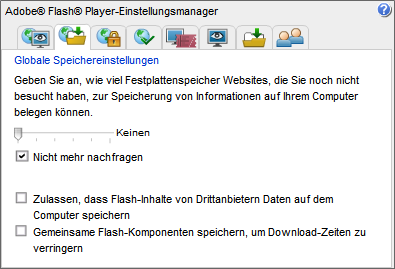
\includegraphics[scale=0.55]{../screenshots/flash1.png}
\caption{Einstellungsmanager f�r Adobe Flash-Player}
\label{abb:flashplayer}
\end{center}
\end{figure}

Wer das Add-on NoScript nutzt, muss zus�tzlich zur aktuellen Webseite dem Server \textit{wwwimages.adobe.com} das Ausf�hren von Javascript erlauben. Anderenfalls funktioniert die Flash-Applikation nicht.
\item Der freie Flash-Player \textbf{Gnash} bietet die M�glichkeit, die Speicherung von Cookies zu konfigurieren. Man klickt mit der rechten Maustaste auf ein Flash-Movie und w�hlt den Punkt \textit{Bearbeiten - Einstellungen} im Kontextmen� und schickt man alle Shared Objects nach /dev/null.

\end{enumerate}


\section{EverCookies}
80\% der Internetnutzer lehnen das Tracking ihres Surfverhaltens ab. Viele Surfer ergreifen einfache Ma�nahmen gegen Tracking Cookies. Nach einer Untersuchung von AdTiger blockieren 52,5\% der Surfer die Annahme von Cookies, die nicht von der aufgerufenen Website stammen (sogenannte Third-Party-Cookies). Andere Studien \footnote{ \href{http://smorgasbork.com/component/content/article/84-a-study-of-internet-users-cookie-and-javascript-settings}{http://smorgasbork.com/component/content/article/84-a-study-of-internet-users-cookie-and-javascript-settings}} kommen auf 15\%...35\% Cookie-Verweigerer unter den Surfern (was mir seri�ser erscheint). Dabei handelt es meist um Surfer, die regelm��ig auf dem Datenhighway unterwegs sind und somit die Erstellung pr�ziser Profile erm�glichen k�nnten. Von Gelegenheits-Surfern kann man kaum umfassenden Interessen-Profile erstellen.\\ 

Die Tracking-Branche reagiert auf diese Entwicklung mit erweiterten Markierungen, die unter der Bezeichnung \textit{EverCookie} zusammengefasst werden. Zus�tzlich zum Tracking-Cookie werden weitere Markierungen im Browser gespeichert. Sp�ter kann ein gel�schtes Tracking-Cookie anhand dieser Markierungen wiederhergestellt werden.\\

Nach empirischen Untersuchungen der University of California \footnote{ \href{http://www.law.berkeley.edu/privacycensus.htm}{http://www.law.berkeley.edu/privacycensus.htm}} nutzen viele Tracking�dienste EverCookie Techniken. H�ufig werden seit 2005 Flash-Cookies bzw. LSOs parallel zu normalen Cookies eingesetzt, wobei diese Technik auf dem absteigenden Ast ist. 2011 nutzen 37\% der TOP100 Webseiten diese Technik, 2012 nur noch 17\%. Die Flash-Cookies werden durch HTML5-Speichertechniken wie DOMstorage ersetzt und ETags. 31\% der TOP100 Webseiten nutzen moderne HTML5-Techniken zur Markierung der Surfer (Stand 2012). 
\begin{itemize}
\item Die \textit{Google-Suche} nutzt DOMstorage, was eine Markierung von Nutzern auch bei deaktivierten Cookies erm�glicht.
\item Die Firma \textit{Clearspring} protzt damit, pr�zise Daten von 250 Mio. Internetnutzern zu haben. Sie setzte bis 2010 Flash-Cookies ein, um gel�schte Cookies wiederherzustellen.
\item \textit{Ebay.de} verwendet Flash-Cookies, um den Browser zu markieren.
\item \textit{AdTiger.de} bietet umfangreiche Angebote zur gezielten Ansprache von Surfern und protzt damit, 98\% der Zugriffe �ber einen Zeitraum von deutlich l�nger als 24h eindeutig einzelnen Nutzern zuordnen zu k�nnen. Nach einer eigenen Studie kann AdTiger aber nur bei 47,5\% der Surfer normale Cookies setzen.
\item Die Firma \textit{KISSmetrics} (\textit{``a revolutionary person-based analytics platform``}) setzte zus�tzlich zu Cookies und Flash-Cookies noch ETags aus dem Cache, DOMStorage und IE-userData ein, um Surfer zu markieren. Aufgrund der negativen Schlagzeilen wird seit Sommer 2011 auf den Einsatz von ETags verzichtet.
\end{itemize}

\subsubsection*{EverCookies - never forget}
Der polnische Informatiker Samy Kamkar hat eine Demonstration \footnote{ \href{http://samy.pl/evercookie/}{http://samy.pl/evercookie/}} von EverCookie Techniken erstellt, die verschiedene technische M�glichkeiten basierend auf HTML5 zeigen:
\begin{itemize}
\item Local Shared Objects (Flash Cookies)
\item Silverlight Isolated Storage
\item Cookies in RGB Werten von automatisch generierten Bildern speichern
\item Cookies in der History speichern
\item Cookies in HTTP ETags speichern
\item Cookies in Browser Cache speichern
\item window.name auswerten
\item Internet Explorer userData Storage
\item Internet Explorer userData Storage
\item HTML5 Database Storage via SQLite
\item HTTP-Auth speichern (zuk�nftig)
\end{itemize}

\subsubsection*{Verteidigungsstrategien}
Zur Verteidigung gibt es drei M�glichkeiten:
\begin{enumerate}
\item Die Verbindung zu Tracking-Diensten kann mit \textbf{AdBlockern} komplett verhindert werden. Es sind Filterlisten zu nutzen, die in der Regel als Privacy Listen bezeichnet werden.
\item Viele EverCookie Techniken nutzen Javascript. Die \textbf{Freigabe von Javascript} nur auf wenigen, vertrauensw�rdigen Seiten sch�tzt ebenfalls.
\item Ein EverCookie-sicherer Browser kann nur mit Konfigurationseinstellungen nicht erreicht werden. Der Datenverkehr ist durch zus�tzliche Ma�nahmen zu reinigen. Bisher kann nur der \textbf{JonDoFox} und der \textbf{JonDoBrowser} alle von Samy Kamkar vorgestellten Techniken w�hrend des Surfens blockieren.
\item Der \textbf{TorBrowser} beseitigt alle Markierungen beim Beenden der Surf-Session (Schlie�en des Browsers oder \textit{Neue Identit�t} im TorButton w�hlen). W�hrend der Session ist man anhand von EverCookies wiedererkennbar. Dieses Verhalten entspricht der Zielstellung der Tor-Entwickler. 
\end{enumerate}

\section{JavaScript}
JavaScript ist eine der Kerntechniken des modernen Internet, birgt aber auch einige Sicherheitsrisiken.
\begin{enumerate}
\item Mit Hilfe von Javascript kann man ein Vielzahl von Informationen �ber den Browser und das Betriebssystem auslesen. Bildschirmgr��e, Farbeinstellungen, installierte Plugins und Hilfs-Applikationen.... Die Website \href{http://browserspy.dk}{http://browserspy.dk} zeigt eine umfangreiche Liste.\\

Diese Informationen k�nnen zu einem individuellen Fingerabdruck verrechnet werden. Anhand dieses Fingerabdruck kann der Surfer wiedererkannt werden, auch wenn er die IP-Adresse mit VPNs oder Anonymisierungsdiensten verschleiert. Die EFF geht davon aus, dass diese Methode von vielen Datensammlern genutzt wird.
\begin{itemize}
 \item \textit{Yahoo! Web Analytics} nutzt Javascript Tracking Code, wenn Cookies blockiert werden.
 \begin{quote}
  \textit{In case Yahoo! Web Analytics cannot set a cookie, the system can still retrieve information from the JavaScript tracking code, the IP address and the web browser user agent. \footnote{ \href{http://help.yahoo.com/l/us/yahoo/ywa/documentation/install\_guide/ig\_get\_started.html}{http://help.yahoo.com/l/us/yahoo/ywa/documentation/install\_guide/ig\_get\_started.html}} }
 \end{quote}  
 \item Ein weiteres Beispiel ist die Firma \textit{bluecave} \footnote{ \href{http://www.bluecava.com}{http://www.bluecava.com}}. Das Trackingscript \textit{BCAL5.js} sammelt Informationen zur verwendeten Software, installierte Schriftarten, Bildschirmgr��e, Browser Plug-ins und ein paar mehr Daten, um daraus einen individuellen Fingerprint zu berechnen. \textit{bluecave} protzt damit, 99\% der Surfer zu erkennen.
 \item Der Trackingdienst Multicounter \footnote{ \href{http://www.multicounter.de/features.html}{http://www.multicounter.de/features.html}} und die Google Suche speichern die per Javascript ausgelesene Bild�schirm�gr��e als individuelles Merkmal.
\end{itemize}

\item Einige EverCookie Techniken nutzen Javascript, um zus�tzliche Markierungen im Browser zu hinterlegen und gel�schte Tracking Cookies wiederherzustellen.

\item Durch Einschleusen von Schadcode k�nnen Sicherheitsl�cken ausgenutzt und der der Rechner kann kompromittiert werden. Das Einschleusen von Schadcode erfolgt dabei auch �ber vertrauensw�rdige Webseiten, beispielsweise mit Cross Site Scripting, wenn diese Websites nachl�ssig programmiert wurden. Werbebanner k�nnen ebenfalls b�s�artigen Javascriptcode transportieren. Im Januar 2013 lieferten die Server des Werbe�netzwerkes OpenX Scripte aus, die Rechner durch Ausnutzung mehrerer Sicherheitsl�cken im Internet Explorer kompromittierten.\footnote{ \href{http://heise.de/-1787511}{http://heise.de/-1787511}}
\end{enumerate}

Ein generelles Abschalten ist heutzutage nicht sinnvoll. �hnlich dem Cookie-Management ben�tigt man ein Whitelisting, welches JavaScript f�r vertrauensw�rdige Websites zur Erreichung der vollen Funktionalit�t erlaubt, im allgemeinen jedoch deaktiviert. Gute Webdesigner weisen den Nutzer darauf hin, dass ohne Javascript eine deutliche Einschr�nkung der Funktionalit�t zu erwarten ist. 



\subsection{NoScript f�r Mozilla Firefox}
Die Einstellungen f�r JavaScript lassen sich mit dem Add-on \textit{NoScript} komfortabel verwalten. Die Erweiterung kann von der Website \footnote{ \href{https://addons.mozilla.org/de/firefox/addon/noscript/}{https://addons.mozilla.org/de/firefox/addon/noscript}} installiert werden. Ein einfacher Klick auf das Download-Symbol startet die Installation. Im Anschluss ist Firefox neu zu starten.\\

\begin{figure}[htb]
\begin{center}
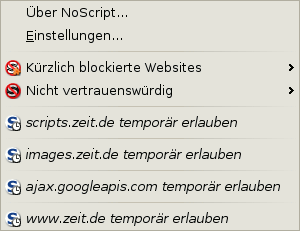
\includegraphics[scale=0.75]{../screenshots/noscript_allow.png}
\caption{NoScript-Button und Men� in der Statuszeile}
\label{abb:noscript_button}
\end{center}
\end{figure}

Nach dem Neustart von Firefox ist in der Statusleiste ein zus�tzliches Symbol vorhanden, welches den Status der Freigabe von JavaScript anzeigt. Ein Klick auf das Symbol �ffnet das im Bild \ref{abb:noscript_button} gezeigte Men�, welches JavaScript f�r die aktuellen Sites generell oder nur tempor�r freigibt.\\

Einige Webseiten verwenden \textit{Captchas} als Spamschutz. Die Captchas werden von Drittseiten eingebunden (Recaptcha.com, Nucaptcha.com...) und funktionieren nur, wenn Javascript f�r den Captcha-Provider freigegeben ist. Wenn das Captcha auf einer Webseite nicht funktioniert, schauen sie in der NoScript-Liste nach, ob evtl. ein Captcha-Provider dabei ist und geben sie Javascript tempor�r f�r diese Domain frei.\\

Weitere Skripte von Drittanbietern werden �blicherweise nur zum Spionieren verwendet und sind f�r die Funktionalit�t selten notwendig.\\

W�hlt man den Punkt \textit{Einstellungen} im NoScript-Men�, �ffnet sich der Einstellungsdialog (Bild \ref{abb:noscript_einst}), der auf dem Reiter \textit{Positivliste} eine Liste der Websites zeigt, f�r welche Java-Script freigegeben wurde. Als Erstes sollte man aus der Positivliste alles entfernen, was man nicht wirklich braucht. In der Liste findet man standardm��ig mit \textit{googlesyndications} auch Surf-Tracker.\\

\begin{figure}[htb]
\begin{center}
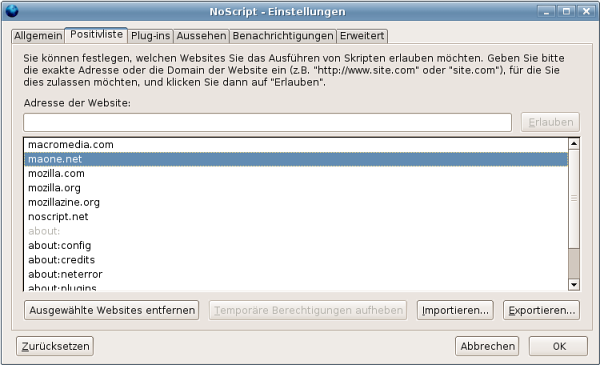
\includegraphics[scale=0.58]{../screenshots/noscript_einst.png}
\caption{Einstellungen f�r NoScript}
\label{abb:noscript_einst}
\end{center}
\end{figure}

Auf dem Reiter \textit{Benachrichtigungen} l�sst sich beispielsweise konfigurieren, ob NoScript den Surfer mit einem Sound oder mit einem Info-Balken dar�ber informiert, dass Scripte auf der aktuellen Webseite blockiert wurden.\\

Der Sound nervt mich, diese Option habe ich deaktiviert. Wenn eine Webseite jedoch nicht wie erwartet funktioniert, kann die kurze Einblendung eines Info-Balkens hilfreich bei der Suche nach den Ursachen sein.\\

NoScript dient nicht nur der Steuerung von Javascript, es bieten \textbf{Schutz gegen vielf�ltige Angriffe} aus dem Netz. (XSS-Angriffe, Webbugs, Click-Hijacking....). Au�erdem blockiert es auch Ping-Attribute und kann f�r eine LIste von Webseiten SSL-Verschl�sselung erzwingen. 

\section{Werbung, HTML-Wanzen und Social Media}
Die auf vielen Websites eingeblendete \textbf{Werbung }wird von wenigen Servern bereitgestellt. Diese nutzen h�ufig (eigentlich immer) die damit gegebenen M�glichkeiten, das Surfverhalten �ber viele Websites hinweg zu erfassen. Mit Hilfe von listen- und musterbasiert Filtern kann der Zugriff auf Werbung sowie die von diesen Servern genutzten Cookies unterbunden werden.\\

Hinweis: Viele Angebote im Web werden �ber Werbung finanziert, da die Nutzer meist nicht bereit sind, f�r diese Angebote zu bezahlen. Die Redaktion von Heise.de hat ein kurzes Statement\footnote{ \href{http://www.heise.de/Adblocker-auf-heise-online-1164703.html}{http://www.heise.de/Adblocker-auf-heise-online-1164703.html}} zu Werbung auf Heise online ver�ffentlicht und erkl�rt, wie sie einzelne Webangebote durch Freigaben im Werbeblocker unterst�tzen k�nnen.\\

Bei \textbf{HTML-Wanzen} (sogenannten Webbugs) handelt es sich um 1x1-Pixel gro�e transparente Bildchen, welche in den HTML-Code einer Webseite oder einer E-Mail eingebettet werden. Sie sind f�r den Nutzer unsichtbar und werden beim Betrachten einer Webseite oder beim �ffnen der E-Mail von einem externen Server geladen und erm�glichen es dem Betreiber des Servers, das Surfverhalten website�bergreifend zu verfolgen.\\

Hinweis: das System METIS\footnote{ \href{http://www.vgwort.de/metis.php}{http://www.vgwort.de/metis.php}} der VG Wort verwendet HTML-Wanzen, um die Besucher von Online-Angeboten zu z�hlen und anhand der Ergebnisse Tantiemen an Autoren auszuzahlen.\\

Facebook und andere Sociale Netze verwenden sogenannte \textbf{Like Buttons}, um Daten zu sammeln. Die Verwendung der Like Buttons ist nach Ansicht von Thilo Weichert (ULD) nicht mit deutschen Datenschutzrecht vereinbar. Deutsche Webseitenbetreiber sind aufgefordert, die Facebook Buttons von ihren Seiten zu entfernen\footnote{ \href{https://www.datenschutzzentrum.de/facebook/}{https://www.datenschutzzentrum.de/facebook}}. Mit dem Aufruf einer Webseite, die den Like Button enth�lt, werden Daten an Facebook �bertragen und dort ausgewertet.\\

Forscher der Universit�t Cambridge (Gro�britannien) konnten im Rahmen einer Untersuchung durch Auswertung der Klicks auf Facebook Like Buttons die sexuelle Orientierung und politische Einstellung der Teilnehmer vorhersagen\footnote{ \href{http://heise.de/-1820638}{http://heise.de/-1820638}}. Man verr�t mit einem Klick auf einen Like Button m�glicherweise Informationen, die man nicht im Netz ver�ffentlichen m�chte. 

\subsection{Tracking-Filter f�r Firefox}
Es gibt mehrere Add-ons f�r Firefox, die Werbung und Trackingelemente blockieren. Das Center for Internet and Society der Stanford Law School hat in einer Analyse vom September 2011 einige L�sungen verglichen \footnote{ \href{https://cyberlaw.stanford.edu/node/6730}{https://cyberlaw.stanford.edu/node/6730}}. Die Ergebnisse in Bild \ref{abb:trackingfilter} zeigen: keine L�sung ist perfekt.\\

\begin{figure}[htb]
\begin{center}
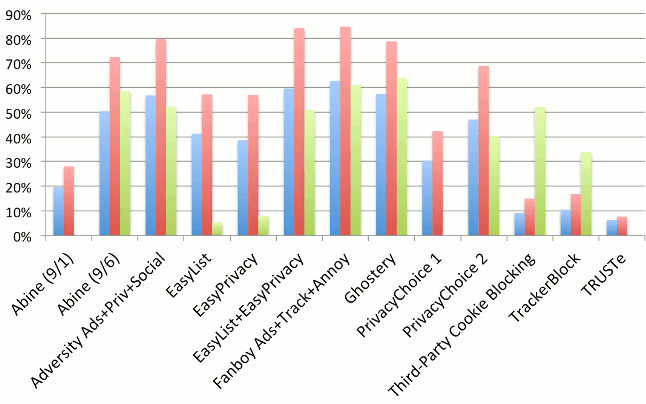
\includegraphics[scale=1.0]{../screenshots/tracking-blocker.png}
\caption{Effektivit�t verschiedener Tracking-Filter}
\label{abb:trackingfilter}
\end{center}
\end{figure}

Aufgrund der Flexibilit�t bei der Einbindung verschiedener Filterlisten empfehle ich \textit{AdBlock Plus}. Mit den Easylist Filterlisten erreichten das Add-on bei dem Test mit die besten Ergebnisse. Die Listen werden st�ndig weiterentwickelt. Es gibt als Zusatz eine spezielle Filterliste f�r deutsche Webseiten.\\

Zus�tzlich zur den Blocklisten\textit{ EasyList+Germany} und \textit{EasyPrivacy} sollte man noch eine Liste abonnieren, die die Social Media Buttons blockiert, z.B. \textit{SocialMediaBlock} von MontzA.\\

\textit{FanBoy} arbeitet seit 2010 mit EasyList zusammen, daher die �hnlich guten Ergebnisse. \textit{Ghostery} schneidet im Test auch gut ab und wird oft empfohlen. Es gibt aber immer wieder Probleme mit Ghostery auf einigen Webseiten, da das Add-on kein Whitelisting kennt. Au�erdem arbeitet es mit einer festen Blockliste, die nicht flexibel erweitert oder kombiniert werden kann. 
\subsection{Adblock f�r Mozilla Firefox}
F�r Mozilla Firefox steht mit \textbf{Adblock Plus}\footnote{ \href{https://addons.mozilla.org/en-US/firefox/addon/adblock-plus/}{https://addons.mozilla.org/en-US/firefox/addon/adblock-plus/}} ein Add-on f�r das listenbasierte Blockieren von Werbung zur Verf�gung. F�r AdBlock Plus gibt es viele Listen zum Blockieren von Werbung (l�nderspezifisch), Tracking-Diensten und der Social Media Like-Buttons. Ein einfacher Klick auf das Install-Symbol der Website startet den Download der Erweiterungen und installiert sie.\\

Nach dem Neustart ist mindestens eine Filterliste zu abonnieren (Bild \ref{abb:adblock1}). Standardm��ig wird f�r deutsche Benutzer die Liste \textit{EasyList Germany + EasyList} vorgeschlagen. \textit{EasyList} ist eine gute Wahl, die man akzeptieren kann.

\begin{figure}[htb]
\begin{center}
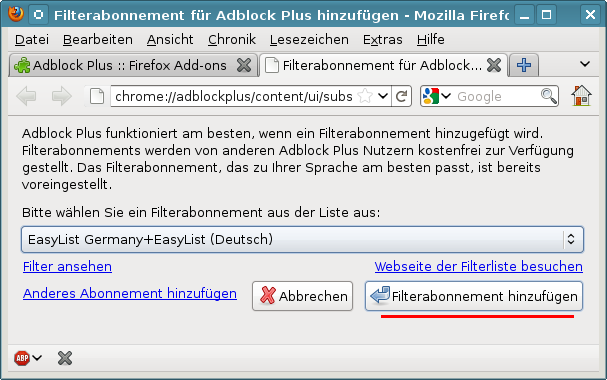
\includegraphics[scale=0.75]{../screenshots/adblock-firststart.png}
\caption{Auswahl einer Liste nach der Installition von Adblock Plus}
\label{abb:adblock1}
\end{center}
\end{figure}

\subsubsection*{Zus�tzliche Filterlisten abonnieren}
Weitere Filterlisten k�nnen im Einstellungen von AdBlock Plus unter dem Men�punkt \textit{Filter Preferences} abonniert werden. Hier ist der Men�punkt \textit{Filter -> Abonnement hinzuf�gen} zu w�hlen. Aus der Liste der angebotenen Filter k�nnen regional passende Listen gew�hlt werden. Folgende Filter-Listen sind als Erg�nzung zur EasyList passend:
\begin{itemize}
 \item \textbf{EasyPrivacy} blockiert meist unsichtbare Tracking-Elemente zum Aussp�hen ihres Verhaltens im Internet mit HTML-Wanzen. Die Liste ist eine sinnvolle Erg�nzung zur EasyList (Germany). Bei der Installation von \textit{EasyPrivacy} kann die zus�tzliche empfohlene EasyList deaktiviert werden, das sie bereits vorhanden ist.
 \item \textbf{SocialMediaBlock} ist eine Liste zum Blockieren der verschiedenen Social Media Tracking Features wie Facebook Like Buttons u.�. Zur Installation kopiert man folgende URL in die Adressleiste von Firefox: \href{abp://subscribe/?location=http://monzta.maltekraus.de/adblock\_social.txt\&title=SocialMediaBlock}{abp://subscribe/?location=http://monzta.maltekraus.de/adblock\_social.txt\&title=SocialMediaBlock}.
\end{itemize}

\subsubsection*{Whitelisting von Websites}
Mit der Version 2.0 hat AdBlock eine Whitelist f�r unaufdringliche Werbung eingef�hrt. Die Filterung wird auf den Webseiten in der Whitelist abgeschaltet, so dass diese Webseiten Werbung einblenden k�nnen. Bisher ist die Whitelist ziemlich leer. Man kann dieses Feature wie in Bild \ref{abb:adblock2} in der �bersicht der Filterlisten abschalten, indem man die Option \textit{Nicht aufdringliche Werbung zulassen} deaktiviert. Alternativ kann man auch das Add-on \textbf{TrueBlock} statt AdBlock verwenden. Es ist 100\% kompatibel mit AdBlock, das Whitelisting ist jedoch standardm��ig deaktiviert. \\

\begin{figure}[htb]
\begin{center}
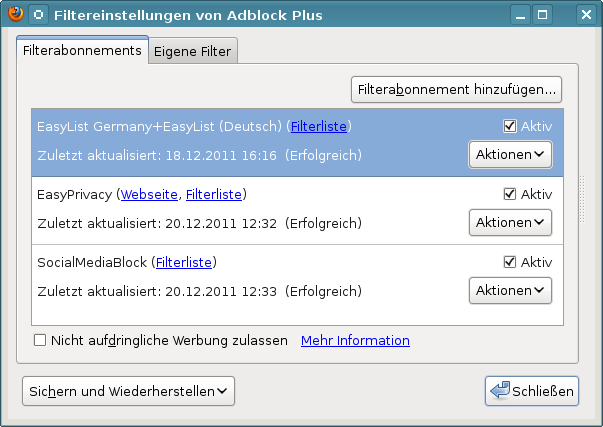
\includegraphics[scale=0.75]{../screenshots/adblock-whitelist.png}
\caption{Whitelisting in AdBlock Plus deaktivieren}
\label{abb:adblock2}
\end{center}
\end{figure}

Statt dessen kann man selbst entscheiden, welchen Webseiten man das Anzeigen von Werbung gestatten m�chte. Mit einem gelegentlichen Klick auf Werbung kann man gute Webseiten bei der Finanzierung unterst�tzen. Wenn Sie eine Webseite im Browser ge�ffnet haben, k�nnen Sie in den Men� von AdBlock die aktuelle Webseite zu einer eigenen Whitelist hinzuf�gen.

\subsubsection*{Vertipper korrigieren}
Die Entwickler von AdBlock sind der Meinung, dass das Korrigieren von Vertippern in der URL ein sinnvolles Feature f�r einen Werbeblocker ist, und haben \textit{URL Fixer} integriert. Die Tippfehlern werden an den Server \textit{urlfixer.org} gesendet und dort gesammelt. Es wird vielen Nutzern nicht gefallen, wenn Daten �ber gerade besuchte Seiten an einen externen Server gesendet werden. Einen Hinweis auf die Daten�bertragung findet man nicht.\\

Man kann dieses (�berfl�ssige) Feature in den Filtereinstellungen von AdBlock auf dem Reiter \textit{Vertipper-Korrekturen} deaktivieren. 

\subsubsection*{Anti-AdBlock}
Anti-AdBlock ist ein Script f�r Webmaster, die den Besucher der Webseite zur Deaktivierung von AdBlock Plus zwingen wollen. Bei aktivem Werbeblocker sieht man beim Besuch einer pr�parierten Webseite nur folgenden Hinweis: 
\begin{center}
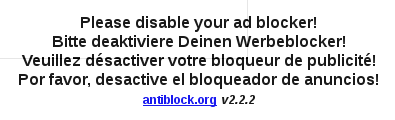
\includegraphics[scale=0.7]{../screenshots/anti-adblock.png}
\end{center}
Wer sich nicht g�ngeln lassen will, kann das Firefox Add-on \textbf{Disable Anti-Adblock}\footnote{ \href{https://addons.mozilla.org/en-US/firefox/addon/disable-anti-adblock/}{https://addons.mozilla.org/en-US/firefox/addon/disable-anti-adblock/}} installieren. Dann kann man die Webseite werbefrei betrachten. 

\section{History Sniffing}
Browser speichern Informationen �ber besuchte Webseiten in einer Surf-History. Eine  empirische Untersuchung der University of California \footnote{ \href{http://cseweb.ucsd.edu/users/lerner/papers/ccs10-jsc.pdf}{http://cseweb.ucsd.edu/users/lerner/papers/ccs10-jsc.pdf}} zeigt, dass ca. 1\% der Top 50.000 Websites versuchen, diese Daten �ber zuvor besuchte Websites auszulesen. Daneben gibt es spezielle Anbieter wie Tealium oder Beencounter, die einem Webmaster in Echtzeit eine Liste der Websites liefern, die ein Surfer zuvor besucht hat. Die dabei �bermittelten Informationen erlauben ein �hnlich detailliertes Interessenprofil zu erstellen, wie das Tracking �ber viele Websites. In der Regel werden die Informationen f�r die Auswahl passender Werbung genutzt.\\

Ein Experiment des Isec Forschungs�labors f�r IT-Sicherheit \footnote{ \href{http://heise.de/-919076}{http://heise.de/-919076}} zeigt, dass diese History-Daten auch zur Deanonymisierung der Surfer genutzt werden k�nnen. Anhand der Browser History wurde ermittelt, welche Gruppen bei Xing der Surfer bisher besucht hat. Da es kaum zwei Nutzer gibt, die zu den gleichen Gruppen geh�ren, konnte mit diesen Daten eine Deanonymiserung erfolgen. Die Realnamen sowie E-Mail Adressen konnten ohne Mithilfe vieler Surfer nur durch den Aufruf der pr�parierten Webseite ermittelt werden.\\

Neben Javascript k�nnen auch CSS-Hacks f�r das Auslesen der Surf-Historie genutzt werden. In der wissenschaftlichen Arbeit \textit{Feasibility and Real-World Implications of Web Browser History Detection} \footnote{ \href{http://www.w2spconf.com/2010/papers/p26.pdf}{http://www.w2spconf.com/2010/papers/p26.pdf}} zeigen Security Experten, wie man die unterschiedliche farbliche Darstellung von bereits besuchten Links auswertet.\\

Die derzeit einzig wirksame Verteidigung besteht in der Deaktivierung der Surf-History. Im Dialog \textit{``Einstellungen``} kann man auf dem Reiter \textit{``Datenschutz''} die Speicherung besuchter Webseiten deaktivieren.

\begin{figure}[htb]
\begin{center}
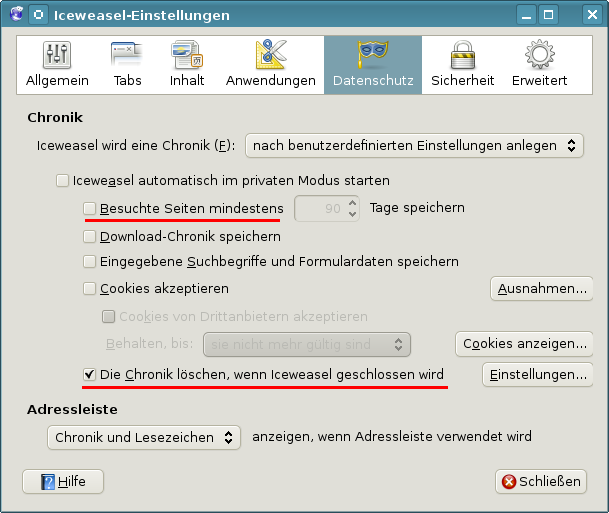
\includegraphics[scale=0.7]{../screenshots/history.png}
\caption{Speichern der Surf-Chronik deaktivieren}
\label{abb:history}
\end{center}
\end{figure}

\section{Browsercache}
Mit jeder aufgerufenen Webseite wird ein ETag gesendet, welches der Browser im Cache speichert. Wird die Webseite erneut aufgerufen, sendet der Browser zuerst das ETag, um zu erfragen, ob die Seite sich ge�ndert hat. Dieses Tag kann eine eindeutige User-ID enthalten. KISSmetrics\footnote{ \href{http://heise.de/-1288914}{http://heise.de/-1288914}} verwendete diese Technik, um gel�schte Tracking-Cookies wieder herzustellen.\\

Ein vollst�ndiges Abschalten des Cache ist nicht empfehlenswert. Man sollte den Cache des Browsers beim Schlie�en automatisch bereinigen. Au�erdem kann man w�hrend des Surfens den Cache usw. mit einer Tastenkombination gelegentlich l�schen.\\

Im Firefox wird der Cache mit weiteren tempor�ren Daten in der \textit{Chronik} zusammengefasst. Die Einstellungen zum L�schen der Chronik findet man unter \textit{Einstellungen} auf dem Reiter \textit{Datenschutz}. Klicken Sie auf den Button \textit{Einstellungen} hinter der Option \textit{Die Chronik l�schen, wenn Firefox geschlossen wird}. In dem sich �ffnenden Dialog kann man detailliert festlegen, welche Daten beim Schlie�en des Browsers gel�scht werden sollen.\\

\begin{figure}[htb]
\begin{center}
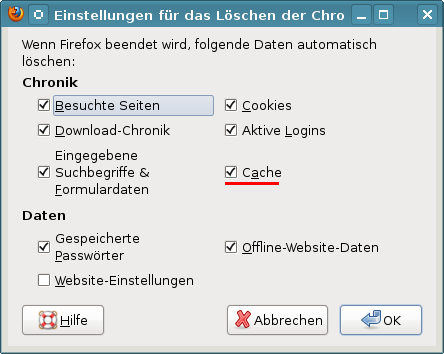
\includegraphics[scale=0.75]{../screenshots/cache_loeschen.png}
\caption{Cache l�schen beim Beenden}
\label{abb:cacheloeschen}
\end{center}
\end{figure}

W�hrend des Surfens kann man die Chronik mit der Tastenkombination STRG-SHIFT-ENTF reinigen oder �ber den Men�punkt \textit{Extra - Neueste Chronik l�schen}.\\

Firefox verwendet einen Cache im Hauptspeicher und einen Disk-Cache auf der Festplatte. Der Cache im Hauptspeicher ist mit 64 MB gro� genug. Den Disk-Cache kann man deaktivieren und damit auch �berfl�ssige Spuren auf dem Rechner vermeiden, die forensisch sichtbar gemacht werden k�nnten. Unter about:config sind daf�r folgende Variablen zu setzen: 
\begin{verbatim}
   browser.cache.disk.enable        false
   browser.cache.disk_cache_ssl     false
   browser.cache.offline.enable     false
\end{verbatim} 

\section{Referer}
Ein Referer liefert die Information, von welcher Seite der Surfer zu der aufgerufenen Webseite gekommen ist, oder bei der Einblendung von Werbung durch Dritte die Information, welche Seite er gerade betrachtet. Es ist ein sehr gut geeignetes Merkmal f�r das Tracking mit Werbung, HTML-Wanzen und Like-Button - die Schleimspur im Web.\\

Die Studie \textit{Privacy leakage vs. Protection measures} \footnote{ \href{http://w2spconf.com/2011/papers/privacyVsProtection.pdf}{http://w2spconf.com/2011/papers/privacyVsProtection.pdf}} zeigt, dass au�erdem viele Web�seiten private Informationen via Referer an Trackingdienste �bertragen. Das folgende Beispiel zeigt den Aufruf eines Werbebanners nach dem Login auf der Webseite http://sports.com
\begin{verbatim}
 GET http://ad.doubleclick.net/adj/....
 Referer: http://submit.sports.com/...?email=name@email.com
 Cookie: id=123456789.....
\end{verbatim}

Mit einer eindeutigen UserID (im Beispiel ein Tracking-Cookie) kann das Surfverhalten �ber viele Webseiten verfolgt werden. Durch zus�tzliche Informationen (im Beispiel eine E-Mail Adresse) werden die gesammelten Datens�tze personalisiert. Im Rahmen der Studie wurde 120 popul�re Webseiten untersucht. 56\% der Webseiten sendeten nach dem Login private Informationen wie E-Mail Adresse, Name oder Wohnort an Trackingdienste.

\subsubsection*{Referer modifizieren f�r Firefox}
Das Add-on \textbf{RefControl} \footnote{ \href{https://addons.mozilla.org/de/firefox/addon/refcontrol/}{https://addons.mozilla.org/de/firefox/addon/refcontrol/}} modifiziert den Referer. Spezifische Einstellungen f�r einzelne Webeiten sind m�glich. Nach der Installation des Plug-Ins sollte im Dialog \textit{Optionen} der Standard-Wert angepasst werden.\\

Die Einstellung \textit{``Blockieren (nur beim Wechsel)``} liefert einen plausiblen Referer,  solange man auf der gleichen Webseite bleibt., entfernt ihn beim Wechsel der Domain. Die Schleimspur wird unterbrochen ohne Funktionen der Website einzuschr�nken.\\

\begin{figure}[htb]
\begin{center}
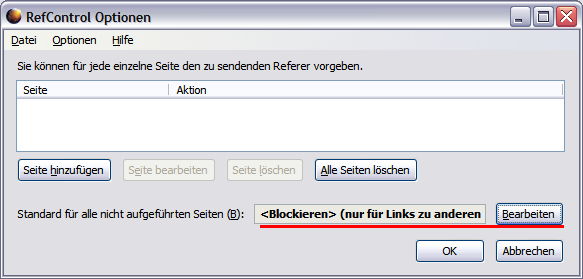
\includegraphics[scale=0.55]{../screenshots/refcontrol1.png}
\caption{Einstellungen von RefControl}
\label{abb:refcontrol}
\end{center}
\end{figure}

Technisch hochentwickelte Datensammler k�nnen den Schutz von RefControl teilweise aushebeln. Google+ und einige Werbenetzwerke �bertragen den Referer zus�tzlich in URL-Parametern. RefControl schadet aber nicht und d�mmere Webmaster tracken auch.

\section{Risiko Plugins}
F�r die Darstellung von Inhalten, die nicht im HTML-Standard definiert sind, kann Firefox Plug-ins nutzen. Popul�r sind Plug-ins f�r die Anzeige von PDF-Dokumenten im Browser oder Flash Videos. Die Nutzung dieser Plug-ins ist jedoch ein Sicherheitsrisiko. Firefox ab Version 14.0 bietet eine einfache M�glichkeit, die Gefahr durch Plug-ins zu reduzieren. Man kann unter der Adresse \textit{about:config} die folgende Variable setzen:
\begin{verbatim}
   plugins.click_to_play  =  true
\end{verbatim} 
Dann werden externe Plug-ins nur aktiviert, wenn der Nutzer es wirklich per Mausklick erlaubt und Drive-By-Download Angriffe sind nicht mehr m�glich.

\subsection{PDF Reader Plugins}
Anwender sind relativ unkritisch gegen�ber PDF-Dokumenten. Was soll beim Anschauen schon passieren? Nur wenige Surfer wissen, dass es mit pr�parierten PDFs m�glich ist, den \textit{ZeuS-Bot} zu installieren und den Rechner zu �bernehmen \footnote{ \href{http://heise.de/-979037}{http://heise.de/-979037}}. 2008 gelang es dem \textit{Ghostnet}, die Rechner�systeme westlicher Regierungen, der US-Regierung und des Dalai Lama mit b�sartigen PDFs zu infizieren \footnote{ \href{http://www.linux-magazin.de/Heft-Abo/Ausgaben/2010/01/Geisterstunde}{http://www.linux-magazin.de/Heft-Abo/Ausgaben/2010/01/Geisterstunde}}. 2012 gelang es dem Trojaner MiniDuke\footnote{ \href{http://heise.de/-1812971}{http://heise.de/-1812971}}, mit b�sartigen PDFs in die Computer von Regierungsorganisationen in Deutschland, Israel, Russland, Gro�britannien, Belgien, Irland, Portugal, Rum�nien, Tschechien und der Ukraine einzudringen. �ber eine von Adobe als \textit{nicht kritisch} eingestufte Sicher�heits�l�cke einer �ber�fl�ssigen PDF-Funktion wurde der Wurm \textit{Win32/Auraax} verteilt \footnote{ \href{http://heise.de/-990544}{http://heise.de/-990544}}...\\

Nach Beobachtung des Sicherheitsdienstleisters Symantec\footnote{ \href{http://heise.de/-981631}{http://heise.de/-981631}} und ScanSafe\footnote{ \href{http://www.scansafe.com/downloads/gtr/2009\_AGTR.pdf}{http://www.scansafe.com/downloads/gtr/2009\_AGTR.pdf}} erfolgen die meisten Angriffe aus dem Web mit b�sartigen PDF-Dokumenten. 2009 wurden f�r ca. 50\% der Angriffe pr�parierten PDF-Dokumente genutzt (mit steigender Tendenz).\\

Schutzma�nahmen: 
\begin{enumerate}
 \item Statt funktions�berladener Monster-Applikationen kann man einfache PDF-Reader nutzen, die sich auf die wesentliche Funktion des Anzeigens von PDF-Dokumenten beschr�nken. Die FSFE stellt auf PDFreaders.org \footnote{ \href{http://www.pdfreaders.org/index.de.html}{http://www.pdfreaders.org/index.de.html}} Open Source Alternativen vor.
\begin{itemize}
 \item F�r Windows werden \textit{Evince} und \textit{Sumatra PDF} empfohlen.
 \item F�r Linux gibt es \textit{Okular} (KDE) und \textit{Evince} (GNOME, XFCE, Unity).
 \item F�r MacOS wird \textit{Vindaloo} empfohlen.
\end{itemize}
\item Wenn die PDF Reader Plugins nicht deinstallierbar sind (keine Adminstrator-Rechte), k�nnen sie im Browser deaktiviert werden. Diese Funktion finden Sie im Addon-Manager unter \textit{Extras -> Add-ons}. PDF-Dokumente sollte man vor dem �ffnen zu speichern und nicht im Kontext des Browsers zu betrachten.
\item Au�erdem sollte man PDF Dokumenten aus unbekannter Quelle ein �hnliches Misstrauen entgegen bringen, wie ausf�hrbaren EXE- oder PAF-Dateien. Man kann einen Online-PDF-Viewer \footnote{ \href{http://view.samurajdata.se/}{http://view.samurajdata.se}} nutzen, um PDF-Dokumente aus dem Internet zu betrachten ohne den eigenen Rechner zu gef�hrden.
\end{enumerate}


\subsection{Java-Applets}
Es gibt eine Vielzahl von sinnvollen Java-Anwendungen. Im Internet spielt Java aber keine Rolle mehr (im Gegensatz zu Javascipt, bitte nicht verwechseln). Trotzdem installiert Oracles Java unter Windows ohne Nachfrage ein Browser-Plugin zum Ausf�hren von Java-Applets, die in Webseiten eingebettet sein k�nnen. Dieses Plug-in ist in erster Linie ein Sicherheitsrisiko und kann zur unbemerkten Installation von Trojanern genutzt werden.\footnote{ \href{http://heise.de/-1485195}{http://heise.de/-1485195}} \footnote{ \href{http://heise.de/-1677249}{http://heise.de/-1677249}} \footnote{ \href{http://heise.de/-1780850}{http://heise.de/-1780850}}\\

Der (Staats-) Trojaner der italienischen Firma \textit{HackingTeam}\footnote{ \href{http://heise.de/-1671203}{http://heise.de/-1671203}} wird beispielsweise mit einer sauber signierten JAR-Datei auf dem Zielsystem installiert. Der Trojaner belauscht Skype, f�ngt Tastatureingaben ab, kann die Webcam zur Raum�berwachung aktivieren und den Standort des Nutzers ermitteln.\\

Als Schutz wird h�ufig die die komplette Deinstallation von Java empfohlen (BSI\footnote{ \href{https://www.bsi.bund.de/ContentBSI/Presse/Pressemitteilungen/Presse2013/Krit\_Schwachstelle\_Java-7-10\_11012013.html}{https://www.bsi.bund.de/ContentBSI/Presse/Pressemitteilungen/Presse2013/Krit\_Schwachstelle\_Java-7-10\_11012013.html}}, DHS\footnote{ \href{http://www.nbcnews.com/technology/technolog/us-warns-java-software-security-concerns-escalate-1B7938755}{http://www.nbcnews.com/technology/technolog/us-warns-java-software-security-concerns-escalate-1B7938755}}, Fefe\footnote{ \href{https://blog.fefe.de/?ts=ae0f1f75}{https://blog.fefe.de/?ts=ae0f1f75}}). Das ist Bullshit und nur sinnvoll, wenn man keine Java-Programme nutzt. Anderenfalls ist die komplette Deinstallation von Java eine unn�tige Einschr�nkung f�r sinnvolle Anwendungen.\\
\begin{itemize}
 \item Aktuelle \textbf{Linux} Distributionen verwenden in der Regel OpenJDK-6/7. Diese Java-JRE installiert KEIN Browser Plug-in. Es besteht also auch keine Gefahr, durch b�sartige Java-Applets aus dem Internet den Rechner zu verseuchen.
 \item Unter \textbf{Windows} bietet die aktuelle Version von Oracles Java die M�glichkeit, die Plug-ins f�r alle Browser unter \textit{Systemsteuerung - Programme - Java} zu deaktivieren (Bild \ref{abb:javadown}).
\begin{figure}[htb]
\begin{center}
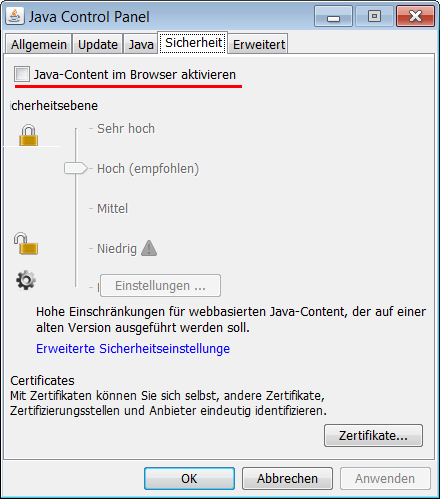
\includegraphics[scale=0.55]{../screenshots/java-ctrl.png}
\caption{Java Plug-in f�r alle Browser deaktivieren}
\label{abb:javadown}
\end{center}
\end{figure}
\end{itemize}

\subsection{Flash und Silverlight}
Auch diese Plugins sind ein Sicherheits- und Privacyrisiko. Sie werden meist f�r die Darstellung von Videos im Web (Youtube) und Panoramadiensten wie Street View (Google) bzw. Street Side (Microsoft) genutzt.\\

Schutzma�nahmen: 
\begin{enumerate}
 \item Das Add-on \textbf{NoScript} kann diese Inhalte blockieren. Es wird ein Platzhalter angezeigt. Bei Bedarf kann man das Video mit einem Mausklick anschauen.
\item Web Videos k�nnen mit Hilfe von Download Sites wie KeepVid \footnote{ \href{http://keepvid.com}{http://keepvid.com}} oder ShareTube \footnote{ \href{http://www.share-tube.de/flvdownload.php}{http://www.share-tube.de/flvdownload.php}} gespeichert und mit einem Mediaplayer abgespielt werden.
\item Die Firefox Add-ons \textbf{UnPlug} \footnote{ \href{https://addons.mozilla.org/en-US/firefox/addon/unplug/}{https://addons.mozilla.org/en-US/firefox/addon/unplug}} oder \textbf{DownloadHelper} \footnote{ \href{https://addons.mozilla.org/de/firefox/addon/video-downloadhelper/}{https://addons.mozilla.org/de/firefox/addon/video-downloadhelper}} k�nnen Videos von vielen Websites herunter laden und dabei in ein gebr�uchlicheres Format f�r Mediaplayer konvertieren.
\end{enumerate}
Wer noch keinen passenden Mediaplayer installiert hat, kann den VideoLAN Player nutzen (VLC-Player), der f�r alle Betriebssysteme zur Verf�gung steht.

\subsection{Weitere Anwendungen}
Neben PDF-Dokumenten k�nnen auch alle anderen Dokument-Typen f�r Drive-by-Donwload Angriffe verwendet werden. Um diese zu unterbinden, sollte man externe Anwendungen f�r Dateien nur nach Best�tigung durch den Anwender �ffnen lassen. Anderenfalls k�nnen Bugs in diesen Anwendungen automatisiert genutzt werden.\\

\begin{figure}[htb]
\begin{center}
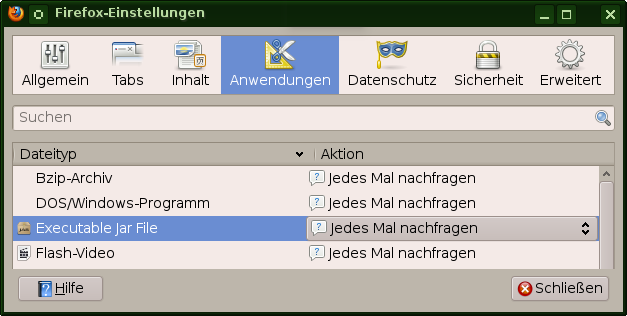
\includegraphics[scale=0.65]{../screenshots/ff-anwendungen.png}
\caption{Externe Anwendungen nur auf Nachfrage �ffnen}
\label{abb:ffhelper}
\end{center}
\end{figure}

Auf dem Reiter \textit{Anwendungen} im Dialog \textit{Einstellungen} k�nnen die Helper-Applications wie im Bild \ref{abb:ffhelper} f�r jeden Dateityp auf \textit{``Jedes Mal nachfragen``} gesetzt werden. Diese Einstellungen sind nat�rlich nur sinnvoll, wenn der Surfer kritisch hinterfragt, ob die Aktion wirklich dem entspricht, was er erwartet. Wer unkritisch bei jeder Nachfrage auf \textit{�ffnen} klickt, muss sich nicht wundern, wenn sein Computer infiziert wird.
\section{HTTPS nutzen}
Viele Websites bieten HTTPS-Verschl�sselung an. Diese sichere Daten�bertragung wird h�ufig nicht genutzt. Mit wenig Konfigurationsaufwand l�sst sich die Nutzung von HTTPS f�r eine definierte Liste von Websites erzwingen.

\subsubsection*{NoScript Enforce HTTPS}
NoScript Enforce HTTPS ist einfach konfigurierbar, kann aber nur \textit{http://} durch \textit{https://} f�r eine Liste von Websites ersetzen. Die Liste muss man per Hand erstellen. Im Dialog \textit{Einstellungen} findet man auf dem Reiter \textit{Erweitert} unter \textit{HTTPS} eine editierbare Liste von Websites.\\

\begin{figure}[htb]
\begin{center}
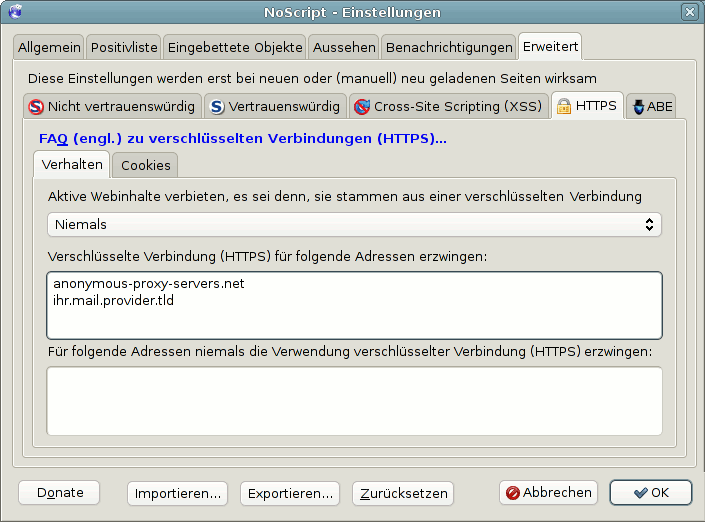
\includegraphics[scale=0.7]{../screenshots/noscript_STS.png}
\caption{Einstellungen f�r NoScript STS}
\label{abb:noscriptsts}
\end{center}
\end{figure}

Standardm��ig ist die Liste leer. Wer das Webinterface eines E-Mail Providers nutzt, sollte die Domain hier eintragen. Au�erdem sollte man die Webseite der Bank eintragen, wenn man Online-Banking nutzt.

\subsubsection*{HTTPS-Everywhere}
Das Firefox Add-on HTTPS-Everywhere\footnote{ \href{https://www.eff.org/https-everywhere}{https://www.eff.org/https-everywhere}} der EFF.org kann auch komplexe Umschreibungen der URLs realisieren, wie es beispw. f�r Wikipedia notwendig ist. Das Add-on bringt aber bereits �ber 2500 Regeln f�r h�ufig genutzte Webseiten mit. Die Konfiguration eigener Regeln ist aufwendiger als bei NoScript und erfolgt �ber XML-Dateien.\\

Bei HTTPS-Everywhere sind Regeln standardm��ig deaktiviert, wenn der Server ein SSL-Zertifikat von CAcert.org nutzt (z.B www.ccc.de) Wenn Sie das Root-Zertifikat von CAcert.org im Browser importiert haben, dann k�nnen Sie diese Regeln in den Einstellungen von HTTPS-Everywhere mit Klick auf das Kreuz aktivieren (Bild \ref{abb:httpseverywherecacert}).

\begin{figure}[htb]
\begin{center}
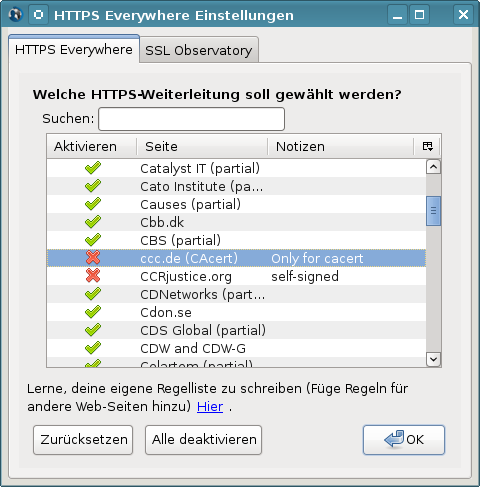
\includegraphics[scale=0.75]{../screenshots/httpseverywhere.png}
\caption{Einstellungen f�r Https-Everywhere}
\label{abb:httpseverywherecacert}
\end{center}
\end{figure}

\subsubsection*{HTTPS-Finder}
Das Add-on HTTPS-Finder\footnote{ \href{https://addons.mozilla.org/de/firefox/addon/https-finder/}{https://addons.mozilla.org/de/firefox/addon/https-finder/}} kann erkennen, ob eine Webseite auch via HTTPS erreichbar ist und erzwingt dann die Nutzung von HTTPS. Es k�nnen automatisch Regeln f�r HTTPS-Everywhere erstellt und aktiviert werden. Das Add-on ist eine gute Erg�nzung f�r HTTPS-Everywhere und erspart das komplexe Erstellen der XML-Dateien von Hand.\\


\section{Vertrauensw�rdigkeit von HTTPS}
IT-Sicherheitsforscher der EFF kommen in einer wissenschaftlichen Arbeit\footnote{ \href{https://eff.org/deeplinks/2010/03/researchers-reveal-likelihood-governments-fake-ssl}{https://eff.org/deeplinks/2010/03/researchers-reveal-likelihood-governments-fake-ssl}} zu dem Schluss, dass Geheim�dienste mit g�ltigen SSL-Zertifikaten schwer erkennbare man-in-the-middle Angriffe durchf�hren k�nnen. Diese Angriffe k�nnen routinem��ig ausgef�hrt werden, schreibt die EFF:
\begin{quote}
 \textit{Certificate-based attacks are a concern all over the world, including in the U.S., since governments everywhere are eagerly adopting spying technology to eavesdrop on the public. Vendors of this technology seem to suggest the attacks can be done routinely.}
\end{quote} 
\begin{enumerate}
 \item Ein erster Angriff dieser Art gegen iranische Internet Nutzer wurde im August 2011 nachgewiesen. Er betraf neben Google die Webdienste mehrerer Geheimdienste (MI6, CIA, Mossad) und au�erdem www.torproject.org. Bei diesem Angriff wurde keine Zertifikate einer standardm��ig vertrauensw�rdigen Certification Authority genutzt, sondern die niederl�ndische Certification Authority DigiNotar wurde gehackt, um g�ltige Zertifikate zu erlangen. Insgesamt wurden 531 SSL-Zertifikate kompromittiert.\footnote{ \href{https://threatpost.com/en\_us/blogs/final-report-diginotar-hack-shows-total-compromise-ca-servers-103112}{https://threatpost.com/en\_us/blogs/final-report-diginotar-hack-shows-total-compromise-ca-servers-103112}}

 \item Neben DigiNotar wurden 2011 die Certification Authorities Comodo, InstantSSL und zwei weitere Sub-Registrare von Comodo erfolgreich angegriffen \footnote{ \href{http://heise.de/-1213999}{http://heise.de/-1213999}}. Die Angreifer konnten sich unbefugt g�ltige Zertifikate f�r die Webseiten von Google, Yahoo, Mozilla und Skype erstellen. Nach Beobachtung des SSL-Observatory der EFF wurden bei den Angriffen mindesten 248 Zertifikate erfolgreich kompromittiert. Auch in diesen F�llen soll der Angriff vom Iran ausgegangen sein.
\end{enumerate}


Die Software f�r einen man-in-the-middle Angriff mit den gef�lschten Zertifikaten gibt es auch als Open Source, z.B. den mitm-proxy\footnote{ \href{http://crypto.stanford.edu/ssl-mitm/}{http://crypto.stanford.edu/ssl-mitm/}} der Stanford University oder dsniff \footnote{ \href{http://www.monkey.org/~dugsong/dsniff/}{http://www.monkey.org/~dugsong/dsniff/}}. Auf der ISS World (Messe f�r �bewachungstechnik) werden fertige Appliances angeboten, gegen Aufpreis auch mit g�ltigem CA-Zertifikat.\\

Wer Kosten (f�r den Aufpreis) oder M�hen (f�r das Hacken einer CA) scheut, kann sich so einfach als Unberechtigter ein g�ltiges SSL-Zertifikat f�r einen Mail- oder Web-Server ausstellen zu lassen \footnote{ \href{https://bugzilla.mozilla.org/show\_bug.cgi?id=556468}{https://bugzilla.mozilla.org/show\_bug.cgi?id=556468}}. Man muss nur einen der zul�ssigen E-Mail Accounts f�r SSL-Admins registrieren und kann ein g�ltiges Fake-Zertifikat erstellen. Par ordre du mufti werden \textit{webmaster\@domain.tld, postmaster\@domain.tld, ssladmin\@domain.tld, ssladministrator\@domain.tld} u.a.m. von den Certification Authorities akzeptiert. Nicht immer sind diese Adressen reserviert und gesch�tzt.

\subsubsection*{Verbesserung der Vertrauensw�rdigkeit von HTTPS}
Es gibt einige M�glichkeiten, die Vertrauensw�rdigkeit der HTTPS-Verschl�sselung zu verbessern und Angriffe mit falschen Zertifikaten zu erschweren.
\begin{itemize}
 \item \textbf{Zertifikate speichern:} Beim ersten Besuch der Webseite wird das SSL-Zertifikat gespeichert. Bei sp�teren Besuchen wird das aktuelle Zertifikat mit dem gespeicherten Zertifikat verglichen. Bei seltsamen Abweichungen wird eine Warnung angezeigt, die der Surfer allerdings bewerten muss. (Firefox Add-ons: Certificate Patrol, JonDoFox)
\item \textbf{Vergleich mit Anderen:} Beim Besuch einer HTTPS-verschl�sselten Webseite wird das Zertifikat mit den Ergebnissen an anderen Punkten der Welt verglichen. Wenn alle Teilnehmer des Netzes das gleiche Zertifikat sehen, ist es wahrscheinlich Ok. Dieser Vergleich kann mit einer zeitlich begrenzten Speicherung kombiniert werden.\\
(Firefox Add-ons:  HTTPS-Everywhere, Perspectives, Convergence.io)\\Obwohl die Idee auf den ersten Blick einleuchtend ist, gibt es einige Probleme bei gro�en Serverfarmen wie Google, Facebook, Amazon, PayPal... Diese Serverfarmen verwenden nicht immer ein einheitliches Zertifikat. Das f�hrt zu Verwirrung bei einem externen Beobachter und zu inkonsistenten Ergebnissen der Notary Server. 

 \item \textbf{Certificate Pinning:} Nur der Betreiber einer Webseite kann wirklich wissen, welche Zertifikate g�ltig sind. Diese Information muss verteilt und ausgewertet werden. Das w�re ein besserer Weg, als der Vergleich mit externen Beobachtern.\\
�ber einen unabh�ngigen Weg wird festgelegt, welche Zertifikate f�r die HTTPS-Verschl�sselung einer Webseite genutzt werden d�rfen. Nur diese Zertifikate werden vom Browser akzeptiert. Google hat die Fingerprints der Zertifikate seiner Webseiten fest im Browser Chrome codiert. Dieses Verfahren skaliert aber nicht. M�glich w�re auch die Nutzung von DNSSEC mittels Sovereign Keys. Brauchbare Ideen zum Certificate Pinning sind noch in der Entwicklung.
\end{itemize}

\subsection{Firefox Add-ons}
Ein paar kleine Erweiterungen f�r Firefox, welche die Vertrauensw�rdigkeit der Zertifikate bei der Nutzung von HTTPS-ver�schl�sselten Verbindungen deutlich erh�hen k�nnen. 

\subsubsection*{HTTPSEverywhere}
HTTPS-Everywhere\footnote{ \href{https://www.eff.org/https-everywhere}{https://www.eff.org/https-everywhere}} kann das SSL-Obervatory der EFF.org nutzen. Wenn man diese Funktion in den Einstellungen des Add-on aktiviert (Bild \ref{abb:sslobservatory}), werden die SSL-Zertifikate der besuchten Webseiten an das SSL-Observatory gesendet. Ist das Zertifikat nicht ok, wird man ab Version 3.0 gewarnt. Es wird eine Datenbasis von weltweit verteilten Nutzern aufgebaut.\\

Hinweis: Aufgrund eines Bug im Proxy-Handling sollte das SSL-Observatory nicht mit dem Anonymisierungsdienst JonDonym genutzt werden. Die Proxy-Einstellungen werden von HTTPSEverywhere ignoriert. In Kombination mit TorButton (TorBrowser) soll dieser Bug nicht auftreten.

\begin{figure}[p]
\begin{center}
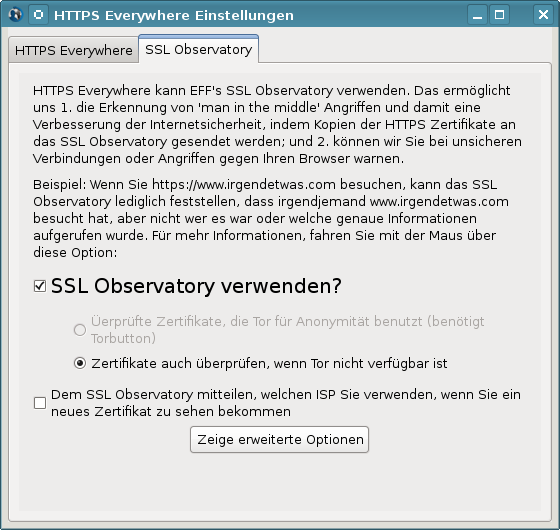
\includegraphics[scale=0.75]{../screenshots/ssl-observatory.png}
\caption{SSL-Observatory aktivieren in HTTPS-Everywhere}
\label{abb:sslobservatory}
\end{center}
\end{figure}

\subsubsection*{Certificates Patrol}
Certificates Patrol \footnote{ \href{https://addons.mozilla.org/de/firefox/addon/certificate-patrol/}{https://addons.mozilla.org/de/firefox/addon/certificate-patrol/}} speichert Informationen zu den Zertifikaten einer Website in einer internen Datenbank. Beim Erstbesuch wird mit einem Informationsbalken am oberen Seitenrand auf ein neues Zertifikat hingewiesen. Man kann es bei Bedarf �berpr�fen. Am einfachsten kann man ein SSL-Zertifikat pr�fen, wenn die Fingerprints vom Webmaster ver�ffentlicht wurden.\\

\begin{figure}[p]
\begin{center}
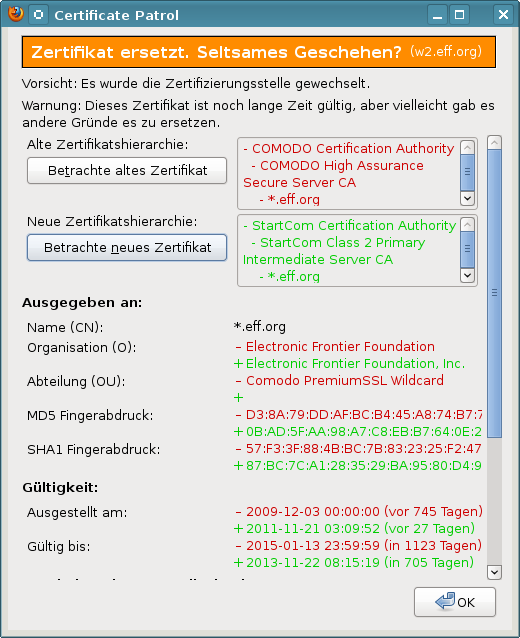
\includegraphics[scale=0.75]{../screenshots/patrol.png}
\caption{Warnung bei setsamen Wechsel des SSL-Zertifikat}
\label{abb:certificatespatrol}
\end{center}
\end{figure}

Hat sich das Zertifikat bei sp�teren Besuchen der Website ge�ndert, zeigt das Add-on Informationen oder Warnungen zum Zertifikatswechsel wie im Bild \ref{abb:certificatespatrol} gezeigt. Der Gefahrenwert wird dabei anhand einer Heuristik ermittelt. Im Beispiel wurde �berraschend ein neues Zertifikat f�r die Webseite der EFF gefunden, obwohl das alte Zertifikat noch lange g�ltig gewesen w�re. Au�erdem wurde die CA gewechselt. Der Nutzer muss bei Warnungen das neue Zertifikat best�tigen, da es ein Hinweis auf einen Angriff sein. Wie kann man pr�fen, ob der Zertifikatswechsel ok ist?
\begin{enumerate}
 \item H�ufig ver�ffentlicht der Webmaster der Seite eine Information zum Zertifikatswechsel im Blog mit den Informationen zum neuen Zertifikat.
 \item Bei Banken u.�. Diensten kann man telefonisch nachfragen, ob das SSL-Zertifikat ge�ndert wurde.
 \item Man kann pr�fen, welches Zertifikat andere Teilnehmer im Netz sehen, beispielsweise mit dem Add-on \textit{Perspectives} (siehe unten). Das Projekt bietet auch eine Demo-Webseite \footnote{ \href{http://data.networknotary.org/notary\_web/notary\_query}{http://data.networknotary.org/notary\_web/notary\_query}}, wo man die Informationen der Notary Server abfragen kann. 
\end{enumerate}

\subsubsection*{Perspectives}
Perspectives\footnote{ \href{https://addons.mozilla.org/en-US/firefox/addon/perspectives/}{https://addons.mozilla.org/en-US/firefox/addon/perspectives/}} vergleicht SSL-Zertifikate mit den bei Notary Servern bekannten Zertifikaten. Wenn alle Notary-Server das gleiche Zertifikat �ber einen l�ngeren Zeitraum sehen, ist es wahrscheinlich g�ltig. Leider gibt es noch nicht viele, international verteilte Notary Server. Alle standardm��ig im Add-on enthaltenen Server werden vom MIT bereit gestellt.\\

Aufgrund der nicht immer eindeutigen Resultate und der Performance der Notary Server ist Perspectives nicht unbedingt f�r eine st�ndige Validierung aller SSL-Zertifikate geeignet. Der Server awxcnx.de ist im Moment nur bei der H�lfte der Notary Server bekannt. Das f�hrt zu einem Fehler bei Perspectives, obwohl eigentlich alles Ok ist.\\

Ich empfehle daher die Abfrage der Notarys bei Bedarf (wenn man ein Zertifikat genauer pr�fen m�chte). Daf�r sind die Einstellungen in den Preferences wie im Bild \ref{abb:perspectives} zu setzen.\\

\begin{figure}[htb]
\begin{center}
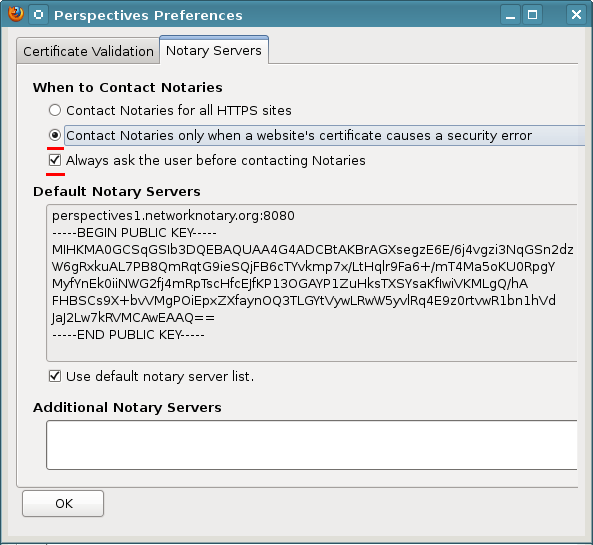
\includegraphics[scale=0.75]{../screenshots/perspectives.png}
\caption{Perspectives Konfiguration}
\label{abb:perspectives}
\end{center}
\end{figure}

Zuk�nftig kann man mit einem Klick der rechten Maustatste auf das Perspectives-Symbol in der Statusleiste einen Check des Zertifikates der Webseite erzwingen und sich die Notary Results anzeigen lassen.\\

\subsubsection*{Convergence.io}
Convergence (Beta): W�hrend Certificate Patrol und Perspectives auf dem alten Zertifikats�system aufsetzen und es etwas verbessern, vollzieht Convergence.io einen radikalen Bruch. Das Add-on ersetzt die Validierung der Zertifikate im Firefox vollst�ndig durch ein eigenes System. Dabei werden �hnlich wie bei Perspectives die Beobachtungen von Notary Server genutzt und mit dem aktuellen Zertifikat verglichen.\\ 

Ich habe (noch) keine Erfahrungen mit Convergence.io gesammelt.

\section{HTTPS Tracking}
Beim Aufbau einer verschl�sselten HTTPS-Verbindung wird eine sogenannte Session initialisert. Die kryptografischen Details sollen an dieser Stelle nicht erl�utert werden.\\

Es ist m�glich, diese HTTPS-Session f�r das Tracking zu nutzen und f�r bis zu 48h immer wieder zu erneuern. Dieses Tracking-Verfahren ist so gut wie nicht nachweisbar, da es voll�st�ndig durch den Webserver realisiert wird und keine Spuren im Browser hinterl�sst. Man kann davon ausgehen, dass dieses Tracking als Erg�nzung zu (Ever-) Cookies genutzt wird. Der Tracking-Service Woopa verwendet seit 2008 HTTPS Session Tracking.\\

F�r HTTPS Session Tracking gibt es zwei M�glichkeiten:
\begin{description}
 \item[Tracking via Session Resumption] ist im RFC 5077 beschrieben.

 Gegen Tracking via Session Resumption kann man sich sch�tzen, indem man im Firefox unter \textit{about:config} die folgende Variable auf FALSE setzt:  
\begin{verbatim}
  security.enable_tls_session_tickets    false  
\end{verbatim} 
Das f�hrt zu geringen Einbu�en der Performance, da f�r jede Seite eine neue SSL-Session ausgehandelt werden muss. Um die Performance-Einbu�en etwas zu kompensieren, kann man \textit{SSL False Start} aktivieren. Dabei werden verschl�sselte Daten bereits gesendet, wenn die Verifizierung der SSL-Session noch nicht abgeschlossen ist. Ein Sicherheitsrisiko besteht dabei nicht. Sollte die Verifizierung der SSL-Session fehlschlagen, werden die bereits empfangenen Daten verworfen.
\begin{verbatim}
  security.ssl.enable_false_start    true  
\end{verbatim}

 \item[Tracking via SSL-Session-ID] wird ebenfalls von allen Webserven unterst�tzt. Auch Webshops k�nnen die Session-ID f�r das Tracking verwenden, z.B. die \textit{xtcModified eCommerce Shopsoftware}\footnote{ \href{http://www.modified-shop.org/wiki/SESSION\_CHECK\_SSL\_SESSION\_ID}{http://www.modified-shop.org/wiki/SESSION\_CHECK\_SSL\_SESSION\_ID}}.\\

Gegen das Tracking via Session-ID sch�tzen nur das TorBrowserBundle und der JonDoBrowser (Beta). Man kann sich nicht durch Konfigurationseinstellungen oder Add-ons sch�tzen, da der Source-Code des Browser daf�r modifiziert werden muss.
 \end{description}




\section{Starke Passw�rter nutzen}
Jeder kennt das Problem mit den Passw�rtern. Es sollen starke Passw�rter sein, sie sollen f�r jede Site unterschiedlich sein und au�erdem soll man sich das alles auch noch merken und auf keinen Fall auf einen Zettel unter der Tastatur ``speichern''. 

\begin{itemize}

\item Was ist ein starkes Passwort? Diese Frage muss man unter Beachtung des aktuellen Stand der Technik beantworten. W�rterbuchangriffe sind ein alter Hut. Das Passwort darf kein Wort aus dem Duden sein, das ist einfach zu knacken. F�r zuf�llige Kombinationen aus Buchstaben, Zahlen und Sonderzeichen kann man Cloud Computing f�r Brute Force Angriffe nutzen. Dabei werden alle m�glichen Kombinationen durchprobiert. Ein 6-stelliges Passwort zu knacken, kostet 0,16 Euro. Eine 8-stellige Kombination hat man mit 400 Euro wahrscheinlich und mit 850 Euro sicher geknackt. Man sollte mindestens 10...12 Zeichen verwenden. (Stand: 2011)

 \item Warum sollte man nicht das gleiche Passwort f�r viele Logins verwenden? Diese Frage beantwortet der Hack von Anonymous gegen HBGary. Den Aktivisten von Anonymous gelang es, Zugang zur User-Datenbank des Content Management Systems der Website zu erlangen. Die Passw�rter konnten geknackt werden. Die Passw�rter wurden vom F�hrungspersonal f�r weiterer Dienste genutzt: E-Mail, Twitter und Linked-In. Die ver�ffentlichten 60.000 E-Mails waren sehr peinlich f�r HBGary \footnote{ 
 \href{http://www.heise.de/ct/artikel/Ausgelacht-1195082.html}{http://www.heise.de/ct/artikel/Ausgelacht-1195082.html}}.
\end{itemize}


Das Add-on \textbf{PwdHash}\footnote{ \href{https://addons.mozilla.org/de/firefox/addon/pwdhash/}{https://addons.mozilla.org/de/firefox/addon/pwdhash/}} vereinfacht den Umgang mit Passw�rtern. Wenn man vor der Eingabe des Passwortes die Taste F2 dr�ckt oder mit einem doppelten @@ beginnt,  wird es in einen einen Hash aus dem Master Passwort und der Domain umgerechnet. Das Ergebnis der Berechnung ist eine 10-stellige zuf�llige Kombination von Buchstaben und Zahlen und wird als Passwort gesendet. Damit ist es m�glich, ein merkbares Master-Passwort f�r alle Sites zu nutzen, bei denen PwdHash funktioniert. Wichtig ist, dass die Domains der Webseiten f�r die �nderung und Eingabe der Passw�rter identisch sind.\\

PwdHash sch�tzt auch vor Phishing-Angriffen. Da die Seite des Phishers von einer anderen Domain geliefert wird, als die originale Website, wird ein falscher Hash generiert, der f�r den Angreifer wertlos ist.\\

Sollte man unterwegs auf einem Rechner das Add-on nicht installiert haben, ist das Login-Passwort nat�rlich nicht zu erraten. Auf der Website des Projektes \footnote{ \href{https://www.pwdhash.com}{https://www.pwdhash.com}} steht der Algorithmus auch als Javascript Applet zur Verf�gung. Man kann sein Master Passwort und die Domain eingeben und erh�lt das generierte Login Passwort. Das kann  man mit Copy \& Paste in das Passwort Eingabefeld �bernehmen.

\subsubsection*{Passwortspeicher}
Passwortspeicher sind kleine Tools, die Username/Passwort Kombinationen und weitere Informationen zu verschiedenen Accounts in einer verschl�sselten Datenbank verwalten. Es gibt mehrere Gr�nde, die f�r die Verwendung eines Passwortspeichers sprechen:
\begin{itemize}
 \item Viele Programme wie Pidgin oder Jitsi speichern Passw�rter unverschl�sselt auf der Festplatte, wenn man die Option zur Speicherung aktiviert (nicht empfohlen!). Andere Programme bieten keinen M�glichkeit zur Speicherung von Passw�rtern, fordern aber die Nutzung einer m�glichst langen, sicheren Passphrase (z.B LUKS oder Truecrypt).
 \item Bei vielen Accounts muss man sich neben Unsername und Passwort weitere Informationen merken wie z.B. die Antwort auf eine Security Frage oder PINs bei Bezahldienstleistern.
 \item In der Regel enthalten Passwortspeicher eine Passwortgenerator, der wirklich zuf�llige und starke Passw�rter generieren kann.
 \item Das Backup wird deutlich vereinfacht. Man muss nur die verschl�sselte Datenbank auf ein externes Backupmedium kopieren.
\end{itemize}

Mir gef�llt \textit{Keypass}\footnote{ \href{http://keypass.en.softonic.com/}{http://keypass.en.softonic.com}} (Windows) bzw. \textit{KeepassX} (Linux) sehr gut. Die Bedienung ist �ber�sichtlich. Man kann Eintr�ge gruppieren, komplizierte Passworte k�nnen �ber die Zwischen�ablage in die Eingabefelder kopiert werden und m�ssen nicht (fehlerhaft) abgetippt werden.
Um krypto�analytische Angriffe zu erschweren, kann man die Datenbank mehrere 10.000x mit AES256 verschl�sseln.\\

\begin{figure}[htb]
\begin{center}
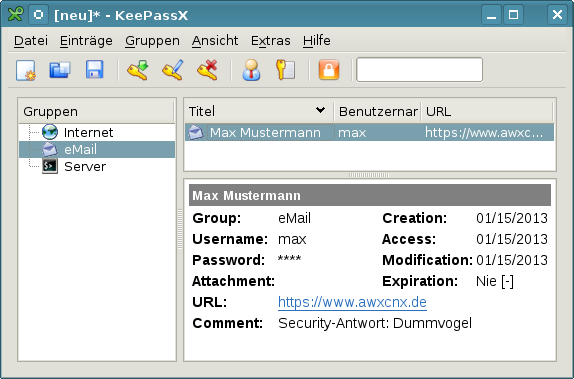
\includegraphics[scale=0.75]{../screenshots/keypass.png}
\caption{KeepassX Hauptfenster}
\label{abb:keypass}
\end{center}
\end{figure}

Einige Passwortspeicher werben mit der M�glichkeit, die Datenbank zwischen verschiedenen Rechnern und Smartphones zu synchronisieren. Dabei wird die Datenbank \textit{in der Cloud} gespeichert. Das ist f�r mich ein Graus, vor allem, weil der geheimdienstliche Zugriff auf Daten \textit{in der Cloud} immer mehr vereinfacht wird.\footnote{ \href{https://www.awxcnx.de/gedanken-bestandsdaten.htm}{https://www.awxcnx.de/gedanken-bestandsdaten.htm}}
\section{HTTP-Header filtern}
Neben der Verwendung von Cookies wird auch der Inhalt des HTTP-Header f�r die Gewinnung von Informationen �ber den Surfer genutzt. Das Projekt \textit{Panopticlick} \footnote{ \href{http://panopticlick.eff.org/}{http://panopticlick.eff.org}} der EFF.org zeigt, dass anhand des Fingerprint des HTTP-Headers 80\% der Surfer eindeutig erkennbar sind. Eine Verkn�pfung dieser Information �ber mehrere Websites hinweg kann eine Verfolgung von Nutzern erm�glichen. Kombiniert man diese Verfolgung mit Daten von Sozialen Netzen (Facebook, Xing), ist eine vollst�ndige Deanonymiserung m�glich.
\begin{itemize}
\item Beispiel \textbf{User-Agent}: Die meisten Browser senden Informationen �ber den verwendeten Browser und das Betriebssystem. Ein Beispiel zeigt, wie detailliert der Browser Auskunft gibt:
\begin{verbatim}
Mozilla/5.0 (Macintosh; U; PPC Mac OS X; de-DE) AppleWebKit/419.3 
(KHTML, like Gecko) Safari/419.3
\end{verbatim}
Beim US-Reiseportal Orbitz werden Surfern mit MacOS (am User-Agent erkennbar) die Hotelzimmer 20-30 Dollar teuerer angeboten, als anderen Kundern\footnote{ \href{http://heise.de/-1626368}{http://heise.de/-1626368}}. Au�erdem k�nnen anhand der Informationen gezielt L�cken in der verwendeten Software ausgenutzt werden.\\


\item Erg�nzende Informationen wie zum Beispiel die bevorzugte \textbf{Sprache}, installierte \textbf{Schrift�arten} und \textbf{Gr��e des Browserfensters} k�nnen einen individuellen Fingerprint des Browsers ergeben. Viele Werte k�nnen per Javascript ausgelesen werden Bei der Google-Suche und beim Trackingdienst Multicounter\footnote{ \href{http://www.multicounter.de/features.html}{http://www.multicounter.de/features.html}} wird die innere Gr��e des Browser�fensters ausgelesen. Die Firma bluecave\footnote{ \href{http://www.bluecava.com/}{http://www.bluecava.com}} nutzt z.B. im Trackingscript \textit{BCAL5.js} u.a. Informationen �ber installierte Schriftarten.\\

Deshalb sollte man Javascript nur f�r vertrauensw�rdige Webseiten erlauben und das Auslesen der Werte behindern (soweit m�glich).
\end{itemize} 


\subsubsection*{Installierte Schriftarten verstecken f�r Firefox}
Um die installierten Schriftarten zu verstecken, deaktiviert man in den Einstellungen die Option \textit{Webseiten das verwenden von eigenen Schriften erlauben}. Man findet die Option in den Firefox \textit{Einstellungen} auf dem Reiter \textit{Inhalt}. Klicken Sie auf den Button \textit{Erweitert}, um im folgenden Dialog Bild \ref{abb:schriftarten} die Option zu deaktivieren.\\

\begin{figure}[htb]
\begin{center}
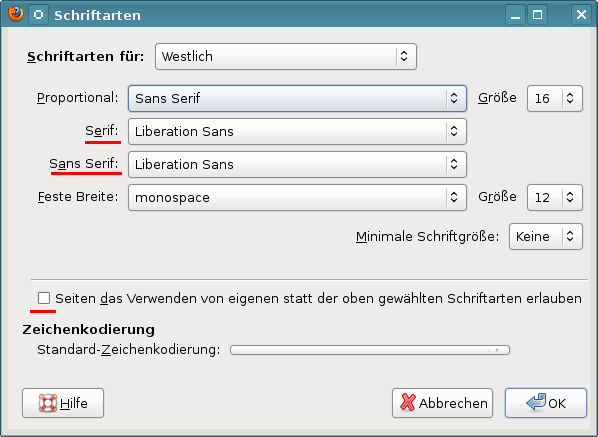
\includegraphics[scale=0.75]{../screenshots/schriftarten.png}
\caption{Schriftarten}
\label{abb:schriftarten}
\end{center}
\end{figure}

Damit kann man nur ''3'' Schriftarten auslesen. Der Browser verwendet aber auch nur die drei Standardschriften zur Darstellung der Webseiten. Damit sehen nicht alle Webseiten exakt so aus, wie es sich der Designer w�nscht. Um die Lesbarkeit zu verbessern, sollten man au�erdem gut lesbare Standardschriften verwenden. Unter Windows eignet sich \textit{Arial}, unter Linux nutzt man am besten \textit{Liberation Sans} (siehe Screenshot).


\subsubsection*{User-Agent modifizieren f�r Firefox}
Es ist nicht so einfach, den User Agent plausibel zu faken. Um durch unsachgem��e �nderung keine eindeutige Kennung zu generieren, sollte man nachdenken, bevor man etwas �ndert.\\

Man kann f�r einen Firefox nur eine andere Firefox-Kennung verwenden. Da die Browser durch individuelle Header erkennbar sind, ist eine Tarnung mit dem User-Agent eines anderen Browsers leicht als Fake zu identifizieren und man ist eindeutig identifizierbar. Einige Firefox Versionen unterscheiden sich nicht nur im User-Agent, sondern auch sehr subtil in einigen anderen HTTP-Headern. Man beachte das Leerzeichen nach dem Komma bei FF 10.0:\\
\begin{verbatim}
 ACCEPT-ENCODING "gzip,deflate"      (Firefox 3.6.x)
 ACCEPT-ENCODING "gzip, deflate"     (Firefox 10.0.x)
\end{verbatim} 

Deshalb muss man auch eine �hnliche Firefox-Version f�r den Fake nutzen, die sich in den �brigen HTTP-Headern nicht unterscheidet.Die meisten Firefox-User nutzen Windows als Betriebssystem. Daher sollte man einen Fake von Firefox f�r Windows nutzen, um in einer gr��eren Anonymt�tsgruppe abzutauchen. F�r Windows Nutzer empfehle ich keine Fakes, da man durch kleine Fehler nur eindeutiger identifizierbar wird.\\

Um die User-Agent Kennung zu �ndern, gibt man in der Adresszeile "about:config" ein und setzt die angebenen Variablen auf die Werte. Alle Werte sind vom Typ \textit{String}. Die folgenden Einstellungen des JonDoFox und TorBrowser kann man f�r Firefox 10.0.x (esr) und auch f�r Firefox 11|12|13 nutzen, wenn man einen ein eher seltenes Betriebssytem nutzt. 

\begin{center}
\begin{tabular}{ll}
Variable & Wert\\
\hline
general.useragent.override & Mozilla/5.0 (Windows NT 6.1; rv:10.0) \\
 & Gecko/20100101 Firefox/10.0\\
\hline
general.appname.override & Netscape\\
general.appversion.override & 5.0 (Windows)\\
general.oscpu.override & Windows NT 6.1\\
general.platform.override & Win32\\
general.productSub.override & 20100101\\
general.buildID.override & 0\\
general.useragent.vendor & \\
general.useragent.vendorSub & \\
\hline
\end{tabular}
\end{center}

Im Firefox 17.0 haben die Mozilla-Entwickler ein paar kleine subtile �nderungen an den gesendeten HTTP-Headern vorgenommen, so dass der Fake des Firefox 10 nicht mehr passt. Bei einem Firefox 17.0 sind folgende Werte zu setzen, um einen plausiblen Fake zu erstellen:

\begin{center}
\begin{tabular}{ll}
Variable & Wert\\
\hline
general.useragent.override & Mozilla/5.0 (Windows NT 6.1; rv:17.0)\\
 & Gecko/17.0 Firefox/17.0\\
\hline
general.appname.override & Netscape\\
general.appversion.override & 5.0 (Windows)\\
general.oscpu.override & Windows NT 6.1\\
general.platform.override & Win32\\
general.productSub.override & 20100101\\
general.buildID.override & 0\\
general.useragent.vendor & \\
general.useragent.vendorSub & \\
\hline
\end{tabular}
\end{center}

\subsubsection*{Geolocation-API deaktivieren}
Mit Hilfe der Geolocation-API kann die geografische Position des Surfer relativ genau bestimmt werden. Zur Ortsbestimmung k�nnen je nach vorhandener Hardware im Rechner die WLANs in der Umgebung genutzt werden, GPS-Hardware oder \dots Im ung�nstigsten Fall kann der Standort nur anhand der IP-Adresse bestimmt werden. Die Nutzung der Geolocation API erfolgt mit Javascript. Da man Javascript auf vielen Seiten frei�geben muss, ist eine Deaktivierung der Geolocation-API sinnvoll. Dann kann ein Webserver den Standort nur relativ ungenau anhand der IP-Adresse ermitteln.\\

Bei Firefox wird die Geoloacation API wird unter \textit{about:config} deaktiviert, indem folgende Variabale auf \textit{FALSE} gesetzt wird:

\begin{verbatim}
   geo.enabled = false
\end{verbatim} 

Diese Einstellung ist wichtig, wenn man die eigene IP-Adresse mit VPNs oder Anonymisierungsdiensten versteckt.

\subsubsection*{Kill Switch f�r Add-ons abschalten}
Die extension blocklist\footnote{ \href{http://https://addons.mozilla.org/en-US/firefox/blocked/}{https://addons.mozilla.org/en-US/firefox/blocked}} kann Mozilla nutzen, um einzelne Add-ons im Browser zu deaktivieren. Es ist praktisch ein kill switch f�r Firefox Add-ons und Plug-ins. Beim Aktualisieren der Blockliste werden detaillierte Informationen zum realen Browser und Betriebssystem an Mozilla �bertragen.

\begin{verbatim}
   https://addons.mozilla.org/blocklist/3/%7Bec8030f7-c20a
   -464f-9b0e-13a3a9e97384%7D/10.0.5/Firefox/20120608001639
   /Linux_x86-gcc3/en-US/default/Linux%202.6.37.6-smp%20
   (GTK%202.24.4)/default/default/20/20/3/
\end{verbatim}

Ich mag es nicht, wenn jemand remote irgendetwas auf meinem Rechner deaktiviert oder deaktivieren k�nnte. Unter \textit{about:config} kann man dieses Feature abschalten:
\begin{verbatim}
   extensions.blocklist.enabled = false
\end{verbatim}

\section{Snakeoil f�r Firefox (�berfl�ssiges)}
Auf der Mozilla-Website f�r Add-ons findet man tausende von Erweiterungen. Man kann nicht alle vorstellen. Ich bekomme immer wieder Hinweise auf dieses oder jenes privacyfreundliche Add-on und habe ein paar Dinge zusammengestellt, die ich nicht in die Empfehlungen aufnehme.\\

Als Grundsicherung empfehle ich die Kombination von \textit{CookieMonster} + \textit{NoScript} + \textit{AdBlock Plus} + \textit{HTTPS   Everywhere} + \textit{RefControl}. Viele Add-ons bieten Funktionen, die von dieser Kombination bereits abgedeckt werden. Andere sind einfach nur �berfl�ssig. 

\subsubsection*{Google Analytics Opt-Out}
Das Add-on von Google verhindert die Ausf�hrung der zu Google-Analytics geh�renden Scripte. Die Scripte werden jedoch trotzdem von den Google Servern geladen und man hinterl�sst Spuren in den Logdaten. Google erh�lt die Informationen zur IP-Adresse des Surfers und welche Webseite er gerade besucht (via Referer). Au�erdem gibt es �ber hundert weitere Surftracker, die ignoriert werden.\\

Die Add-ons NoScript und AdBlock erledigen diese Aufgabe besser.
Kategorie: \textit{echtes Snakeoil}

\subsubsection*{GoogleSharing}
Das Add-on verteilt alle Anfragen an die Google-Suche, Google-Cookies usw. �ber zentrale Server an zuf�llig ausgew�hlte Nutzer von GoogleSharing. Die Ergebnisse werden von den zuf�llig ausgew�hlten Nutzern �ber die zentralen Server zur�ck an den lokalen Firefox geliefert.\\

Nach unserer Meinung verbessert man seine Privatsph�re nicht, indem die Daten einem weiteren Dienst zur Verf�gung stellt. Das der eigene Rechner dabei auch unkontrolliert Daten von anderen Nutzern stellvertretend an Google weiterleitet, ist ein unn�tiges Risiko. Google speichert diese Informationen und gibt sie breitwillig an Beh�rden und Geheimdienste weiter. So kann man unschuldig in Verwicklungen geraten, die amn lieber vermeiden m�chte. Bei daten-speicherung.de findet man aktuelle Zahlen zur Datenweitergabe von Google an Beh�rden und Geheimdienste: 
\begin{itemize}
 \item 3x t�glich an deutsche Stellen
 \item 20x t�glich an US-amerikanische Stellen
 \item 6x t�glich an britische Stellen
\end{itemize}

Statt GoogleSharing sollte man lieber privacy-freundliche Alternativen nutzen: die Suchmaschine Ixquick.com oder Startingpage.com, f�r E-Mails einen Provider nutzen, der den Inhalt der Nachrichten nicht indexiert, openstreetmap.org statt Google-Maps verwenden\dots
Kategorie: \textit{gef�hrliches Snakeoil} 

\subsubsection*{Zweite Verteidigungslinie?}
Eine Reihe von Add-ons bieten Funktionen, welche durch die oben genannte Kombination bereits abgedeckt werden: 
\begin{itemize}
 \item \textit{FlashBlock} blockiert Flash-Animationen. Das erledigt auch NoScript.
 \item \textit{ForceHTTPS} kann f�r bestimmte Webseiten die Nutzung von HTTPS erzwingen, auch diese Funktion bietet NoScript.
 \item \textit{Targeted Advertising Cookie Opt-Out} und \textit{Ghostery} blockieren Surftracker. Es werden Trackingdienste blockiert, die auch AdBlock Plus mit der \textit{EasyPrivacy Liste} sehr gut blockiert. Au�erdem gibt es immer wieder Probleme mit \textit{Ghostery} auf einigen Webseiten, da das Add-on kein Whitelisting kennt.
 \item \textit{No FB Tracking} blockiert die Facebook Like Buttons. Auch das kann AdBlock Plus besser. Die SocialMediaBlock Liste von MontzA blockieren nicht nur Facebook Like Buttons sondern andere Social Networks.
 \item 
\end{itemize}

Wer meint, es nutzen zu m�ssen - Ok.

 
\end{document}